\documentclass[12pt]{article}
\usepackage[amsmath]{e-jc}
\usepackage{graphicx}
\usepackage{tikz}
\usepackage{booktabs}
\usepackage[shortlabels]{enumitem}
\setlength{\emergencystretch}{2em}

\definecolor{kgray}{HTML}{AAAAAA}
\definecolor{kyellow}{HTML}{FFF64C}
\definecolor{kred}{HTML}{FF6666}
\definecolor{kblue}{HTML}{4A86E8}
\tikzset{
  lab/.style={font=\scriptsize,text=black!55},
  capt/.style={font=\small},
}

\newcommand{\seqnum}[1]{\href{https://oeis.org/#1}{\underline{#1}}}
\newcommand{\kA}{\mathsf{A}}
\newcommand{\kB}{\mathsf{B}}
\newcommand{\kC}{\mathsf{C}}
\newcommand{\kE}{\mathsf{E}}
\newcommand{\ZZ}{\mathbb{Z}}
\newcommand{\strip}{\Sigma_h}
\newcommand{\tmax}{{\tau^*}}

\dateline{TBD}{TBD}{TBD}
\MSC{05C35, 05D40, 52C05, 68V05}
\Copyright{The author. Released under the CC BY license (International 4.0).}

\title{The maximum size of a blackout that keeps\\ every lattice rectangle identifiable}

\author{Arjun Pemmasani}
\authortext{}{Department of Mathematics, Harvey Mudd College, Claremont, California, USA
(\email{apemmasani@hmc.edu}).}

\begin{document}

\maketitle

\begin{abstract}
Black out some points of an $h\times m$ grid. The blackout is valid if every rectangle with
corners in the grid, tilted or not, is determined by its white corners. Kagey asked for the
largest size $f(h,m)$ of a valid blackout. For axis-aligned rectangles alone this is a
Tur\'an problem for bipartite graphs without cycles of length $4$ and $6$, and a bound of
Neuwirth gives $f(h,m)\le m+\lfloor h^2/4\rfloor$ for $m\ge3$. Let $m_h$ be the least width
from which equality always holds. We prove that
$\lfloor h^2/4\rfloor\le m_h\le h^{2+o(1)}$ for every height $h\ge4$. The upper bound places
the columns that contain two black points at random and uses the local lemma. The same
construction gives a lower bound for $f(h,m)$ at every width. An explicit construction
gives equality for every $h\ge3$ and every $m\ge h^4/16+O(h^3)$. We also determine
$f(h,m)$ for every $h\le6$ and every $m$, and for $h=7$ and $m\ge24$. Some of these small
values rest on computer checks with verified certificates.
\end{abstract}

\section{Introduction}\label{sec:intro}

Start with an $h\times m$ grid of points and black out some of them. A game master then
chooses a rectangle with corners in the grid, possibly a tilted one, and tells us which of
its corners are white. The blackout is \emph{valid} if this always determines the rectangle
(Definition~\ref{def:valid}). Kagey~\cite{kagey001} asks for the largest size
$f(h,m)$ of a valid blackout. Figure~\ref{fig:game} shows one round. The known values of
$f(h,m)$ are sequence \seqnum{A397315} in the OEIS.

\begin{figure}[ht]
\centering
\resizebox{0.5\textwidth}{!}{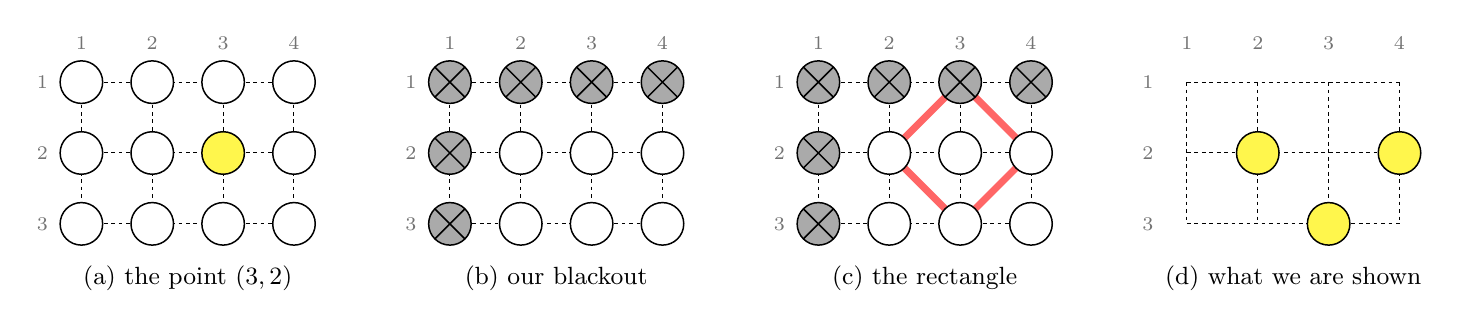
\begin{tikzpicture}[x=0.9cm,y=0.9cm,baseline=(current bounding box.north)]
  \begin{scope}[xshift=0.000cm]
    \draw[black,line width=0.36pt,dash pattern=on 1.35pt off 1.35pt] (1,-1) -- (4,-1) (1,-2) -- (4,-2) (1,-3) -- (4,-3) (1,-1) -- (1,-3) (2,-1) -- (2,-3) (3,-1) -- (3,-3) (4,-1) -- (4,-3);
    \filldraw[fill=white,draw=black,line width=0.54pt] (1,-1) circle (0.3);
    \filldraw[fill=white,draw=black,line width=0.54pt] (2,-1) circle (0.3);
    \filldraw[fill=white,draw=black,line width=0.54pt] (3,-1) circle (0.3);
    \filldraw[fill=white,draw=black,line width=0.54pt] (4,-1) circle (0.3);
    \filldraw[fill=white,draw=black,line width=0.54pt] (1,-2) circle (0.3);
    \filldraw[fill=white,draw=black,line width=0.54pt] (2,-2) circle (0.3);
    \filldraw[fill=kyellow,draw=black,line width=0.54pt] (3,-2) circle (0.3);
    \filldraw[fill=white,draw=black,line width=0.54pt] (4,-2) circle (0.3);
    \filldraw[fill=white,draw=black,line width=0.54pt] (1,-3) circle (0.3);
    \filldraw[fill=white,draw=black,line width=0.54pt] (2,-3) circle (0.3);
    \filldraw[fill=white,draw=black,line width=0.54pt] (3,-3) circle (0.3);
    \filldraw[fill=white,draw=black,line width=0.54pt] (4,-3) circle (0.3);
    \node[lab] at (1,-0.45) {1};
    \node[lab] at (2,-0.45) {2};
    \node[lab] at (3,-0.45) {3};
    \node[lab] at (4,-0.45) {4};
    \node[lab] at (0.45,-1) {1};
    \node[lab] at (0.45,-2) {2};
    \node[lab] at (0.45,-3) {3};
    \node[capt,anchor=north] at (2.50,-3.45) {(a) the point $(3,2)$};
  \end{scope}
  \begin{scope}[xshift=4.680cm]
    \draw[black,line width=0.36pt,dash pattern=on 1.35pt off 1.35pt] (1,-1) -- (4,-1) (1,-2) -- (4,-2) (1,-3) -- (4,-3) (1,-1) -- (1,-3) (2,-1) -- (2,-3) (3,-1) -- (3,-3) (4,-1) -- (4,-3);
    \filldraw[fill=kgray,draw=black,line width=0.54pt] (1,-1) circle (0.3);
    \draw[black,line width=0.54pt] (0.788,-0.788) -- (1.212,-1.212) (0.788,-1.212) -- (1.212,-0.788);
    \filldraw[fill=kgray,draw=black,line width=0.54pt] (2,-1) circle (0.3);
    \draw[black,line width=0.54pt] (1.788,-0.788) -- (2.212,-1.212) (1.788,-1.212) -- (2.212,-0.788);
    \filldraw[fill=kgray,draw=black,line width=0.54pt] (3,-1) circle (0.3);
    \draw[black,line width=0.54pt] (2.788,-0.788) -- (3.212,-1.212) (2.788,-1.212) -- (3.212,-0.788);
    \filldraw[fill=kgray,draw=black,line width=0.54pt] (4,-1) circle (0.3);
    \draw[black,line width=0.54pt] (3.788,-0.788) -- (4.212,-1.212) (3.788,-1.212) -- (4.212,-0.788);
    \filldraw[fill=kgray,draw=black,line width=0.54pt] (1,-2) circle (0.3);
    \draw[black,line width=0.54pt] (0.788,-1.788) -- (1.212,-2.212) (0.788,-2.212) -- (1.212,-1.788);
    \filldraw[fill=white,draw=black,line width=0.54pt] (2,-2) circle (0.3);
    \filldraw[fill=white,draw=black,line width=0.54pt] (3,-2) circle (0.3);
    \filldraw[fill=white,draw=black,line width=0.54pt] (4,-2) circle (0.3);
    \filldraw[fill=kgray,draw=black,line width=0.54pt] (1,-3) circle (0.3);
    \draw[black,line width=0.54pt] (0.788,-2.788) -- (1.212,-3.212) (0.788,-3.212) -- (1.212,-2.788);
    \filldraw[fill=white,draw=black,line width=0.54pt] (2,-3) circle (0.3);
    \filldraw[fill=white,draw=black,line width=0.54pt] (3,-3) circle (0.3);
    \filldraw[fill=white,draw=black,line width=0.54pt] (4,-3) circle (0.3);
    \node[lab] at (1,-0.45) {1};
    \node[lab] at (2,-0.45) {2};
    \node[lab] at (3,-0.45) {3};
    \node[lab] at (4,-0.45) {4};
    \node[lab] at (0.45,-1) {1};
    \node[lab] at (0.45,-2) {2};
    \node[lab] at (0.45,-3) {3};
    \node[capt,anchor=north] at (2.50,-3.45) {(b) our blackout};
  \end{scope}
  \begin{scope}[xshift=9.360cm]
    \draw[black,line width=0.36pt,dash pattern=on 1.35pt off 1.35pt] (1,-1) -- (4,-1) (1,-2) -- (4,-2) (1,-3) -- (4,-3) (1,-1) -- (1,-3) (2,-1) -- (2,-3) (3,-1) -- (3,-3) (4,-1) -- (4,-3);
    \draw[kred,line width=2.55pt,line join=round] (2,-2) -- (3,-1) -- (4,-2) -- (3,-3) -- cycle;
    \filldraw[fill=kgray,draw=black,line width=0.54pt] (1,-1) circle (0.3);
    \draw[black,line width=0.54pt] (0.788,-0.788) -- (1.212,-1.212) (0.788,-1.212) -- (1.212,-0.788);
    \filldraw[fill=kgray,draw=black,line width=0.54pt] (2,-1) circle (0.3);
    \draw[black,line width=0.54pt] (1.788,-0.788) -- (2.212,-1.212) (1.788,-1.212) -- (2.212,-0.788);
    \filldraw[fill=kgray,draw=black,line width=0.54pt] (3,-1) circle (0.3);
    \draw[black,line width=0.54pt] (2.788,-0.788) -- (3.212,-1.212) (2.788,-1.212) -- (3.212,-0.788);
    \filldraw[fill=kgray,draw=black,line width=0.54pt] (4,-1) circle (0.3);
    \draw[black,line width=0.54pt] (3.788,-0.788) -- (4.212,-1.212) (3.788,-1.212) -- (4.212,-0.788);
    \filldraw[fill=kgray,draw=black,line width=0.54pt] (1,-2) circle (0.3);
    \draw[black,line width=0.54pt] (0.788,-1.788) -- (1.212,-2.212) (0.788,-2.212) -- (1.212,-1.788);
    \filldraw[fill=white,draw=black,line width=0.54pt] (2,-2) circle (0.3);
    \filldraw[fill=white,draw=black,line width=0.54pt] (3,-2) circle (0.3);
    \filldraw[fill=white,draw=black,line width=0.54pt] (4,-2) circle (0.3);
    \filldraw[fill=kgray,draw=black,line width=0.54pt] (1,-3) circle (0.3);
    \draw[black,line width=0.54pt] (0.788,-2.788) -- (1.212,-3.212) (0.788,-3.212) -- (1.212,-2.788);
    \filldraw[fill=white,draw=black,line width=0.54pt] (2,-3) circle (0.3);
    \filldraw[fill=white,draw=black,line width=0.54pt] (3,-3) circle (0.3);
    \filldraw[fill=white,draw=black,line width=0.54pt] (4,-3) circle (0.3);
    \node[lab] at (1,-0.45) {1};
    \node[lab] at (2,-0.45) {2};
    \node[lab] at (3,-0.45) {3};
    \node[lab] at (4,-0.45) {4};
    \node[lab] at (0.45,-1) {1};
    \node[lab] at (0.45,-2) {2};
    \node[lab] at (0.45,-3) {3};
    \node[capt,anchor=north] at (2.50,-3.45) {(c) the rectangle};
  \end{scope}
  \begin{scope}[xshift=14.040cm]
    \draw[black,line width=0.36pt,dash pattern=on 1.35pt off 1.35pt] (1,-1) -- (4,-1) (1,-2) -- (4,-2) (1,-3) -- (4,-3) (1,-1) -- (1,-3) (2,-1) -- (2,-3) (3,-1) -- (3,-3) (4,-1) -- (4,-3);
    \filldraw[fill=kyellow,draw=black,line width=0.54pt] (2,-2) circle (0.3);
    \filldraw[fill=kyellow,draw=black,line width=0.54pt] (4,-2) circle (0.3);
    \filldraw[fill=kyellow,draw=black,line width=0.54pt] (3,-3) circle (0.3);
    \node[lab] at (1,-0.45) {1};
    \node[lab] at (2,-0.45) {2};
    \node[lab] at (3,-0.45) {3};
    \node[lab] at (4,-0.45) {4};
    \node[lab] at (0.45,-1) {1};
    \node[lab] at (0.45,-2) {2};
    \node[lab] at (0.45,-3) {3};
    \node[capt,anchor=north] at (2.50,-3.45) {(d) what we are shown};
  \end{scope}
\end{tikzpicture}
}
\caption{One round on a largest valid blackout of the $3\times4$ grid. Points are
(column, row). Gray crossed circles are black. Panel (c) shows the red rectangle, and (d)
its white corners.}
\label{fig:game}
\end{figure}

Throughout the paper we put $q_h=\lfloor h^2/4\rfloor$ and
$W_h=1+\lfloor (h-1)^2/4\rfloor$.

We first look at the axis-aligned rectangles alone. Record a blackout $S$ by its
\emph{row-column graph} $G_S$, the bipartite graph that joins row $j$ to column $i$ when
the point in column $i$ and row $j$ is black. For $m\ge3$, the blackout distinguishes all
axis-aligned rectangles exactly when $G_S$ has no cycle of length $4$ or $6$
(Lemma~\ref{lem:girth}). Hence $|S|$ is at most the largest number of edges of a bipartite
graph of girth at least $8$ with parts of sizes $h$ and $m$. Neuwirth
\cite[Theorem~1(ii) and Proposition~17]{neuwirth2001} proved that this number is at most
$m+q_h$ when $m\ge q_h$, and that it is attained by the following graph. Take a complete
bipartite graph on the $h$ rows with parts as equal as possible. Subdivide each of its
$q_h$ edges by a column, and join every remaining column to one row. In the grid, this
means that $q_h$ columns contain 2 black points, on $q_h$ different row pairs, and that
every other column contains 1 black point. We call such columns \emph{doubles} and
\emph{singletons}. So $f(h,m)\le m+q_h$ for $m\ge3$ (Theorem~\ref{thm:rowbound}).

The graph $G_S$ does not see the order of the columns, but the tilted rectangles do. Hence
the problem for all rectangles is a problem about embeddings. We must order the columns of
a subdivided triangle-free graph with pendant leaves, and choose the rows of the leaves, so
that no 2 rectangles of the grid show the same white corners. Our main result says that
this is possible at every height once the width is a little more than $h^2$, and that it
is not possible for widths below $q_h$.

For $h\ge3$ let $m_h$ be the least integer $M\ge1$ such that $f(h,m)=m+q_h$ for every
$m\ge M$. We do not know whether $f(h,m+1)\ge f(h,m)+1$ always holds. Hence equality at one
width does not obviously give equality at the next width, and this is why we define $m_h$
through all larger widths. Write $\tau(n)$ for the number of divisors of $n$, and put
$\tmax(h)=\max\{\tau(n):1\le n\le h^2\}$.

\begin{theorem}[the threshold]\label{thm:threshold}
For every $h\ge3$ the number $m_h$ exists.
\begin{enumerate}[(a)]
\item For every $h\ge4$ we have $m_h\ge q_h$.
\item There is an absolute constant $C$ such that $m_h\le C\,h^2\,\tmax(h)^2$ for every
$h\ge3$.
\end{enumerate}
In particular, for every $\varepsilon>0$ there is a constant $C_\varepsilon$ with
$q_h\le m_h\le C_\varepsilon h^{2+\varepsilon}$ for every $h\ge4$.
\end{theorem}

Part (a) holds because equality needs $q_h$ doubles (Corollary~\ref{cor:small-m}). For
part (b) we use the odd and the even rows as the 2 parts. For even $h$ every singleton is
black in row $1$ or row $h$. For odd $h$ we use up to 4 blocks of columns, each with its
own 2 rows for the singletons. We then choose the columns of the doubles independently at
random in a window of length about $q_h\,\tmax(h)^2$. A confusion between 2 rectangles
needs a few black points in a special position, and for fixed rows a divisor function
bounds the number of such positions. The local lemma gives columns with no confusion that
involves 2 or more doubles. The other confusions are removed by fixing the singletons in a
few columns near each double. The last statement of the theorem follows from
$\tau(n)\le K_\delta n^\delta$ \cite[Theorem~315]{hardywright2008}. The same construction
with fewer doubles gives a lower bound at every width.

\begin{corollary}[every width]\label{cor:everywidth}
There is an absolute constant $C'$ such that, for every $h\ge3$ and every $m\ge1$,
\[
 f(h,m)\ \ge\ m+\min\Bigl(q_h,\Bigl\lfloor\frac{m}{C'\,\tmax(h)^2}\Bigr\rfloor\Bigr).
\]
\end{corollary}

This improves on the bound $f(h,m)\ge m+h-1$ of Lemma~\ref{lem:cross} only for
$m\ge C'h\,\tmax(h)^2$, and it adds nothing for $h\le8$. The constants are large
(Remark~\ref{rem:constants}), so we also give an explicit construction.

\begin{proposition}[explicit construction]\label{thm:general}
Let $h\ge3$ and put $M_h=q_h+(q_h-1)W_h$. Then $f(h,m)=m+q_h$ for every $m\ge M_h$. Hence
$m_h\le M_h=h^4/16+O(h^3)$.
\end{proposition}

Here the doubles are $W_h+1$ columns apart. The singletons are black in row $1$ or in
row $h$, and they switch between these 2 rows at every double (Figure~\ref{fig:seas}).

\begin{theorem}[small heights]\label{thm:small}
For $2\le h\le7$ and $m\ge\max(h,3)$, the values of $f(h,m)-m$ are those in
Table~\ref{tab:values}.
\end{theorem}

\begin{table}[ht]
\centering
\begin{tabular}{@{}cl@{}}
\toprule
$h$ & $f(h,m)-m$ for $m\ge\max(h,3)$\\
\midrule
$2$ & $1$\\
$3$ & $2$\\
$4$ & $3$ for $m=4,5$, and $4$ for $m\ge6$\\
$5$ & $5$ for $5\le m\le7$, and $6$ for $m\ge8$\\
$6$ & $6$ for $m=6,7$, $7$ for $8\le m\le11$, $8$ for $12\le m\le14$, and $9$ for
$m\ge15$\\
$7$ & $7$ for $m=7$, $8$ for $m=8$, and $12$ for $m\ge24$ (see Remark~\ref{rem:seven} for $m\ge21$)\\
\bottomrule
\end{tabular}
\caption{The values of Theorem~\ref{thm:small}. The last value in each row is $q_h$.}
\label{tab:values}
\end{table}

Since $f(h,m)=f(m,h)$, $f(1,m)=m$, and $f(2,2)=4$, this determines $f(h,m)$ for every
$h\le6$ and every $m$. It gives $m_4=6$, $m_5=8$, $m_6=15$, and $m_7\le24$, while
$q_h=4,6,9,12$ for these heights. The rows $h\le3$ and the values $f(4,m)=m+4$ for $m\ge6$
are proved by hand. The value $f(3,m)=m+2$ was first proved in Lean by the Omega
Institute~\cite{trureturing2026}. All other entries are computer-assisted. Their lower
bounds are explicit blackouts. For $h\ge5$ the largest value is attained by one blackout
extended by columns with 1 black point in a fixed row, and we reduce the validity of all
extensions to one finite check (Theorem~\ref{thm:collar}). Their
upper bounds below $m+q_h$ are unsatisfiable SAT instances with checked LRAT certificates
(Section~\ref{sec:verify}).

\paragraph{Related work.} Choosing white points that distinguish all rectangles is a test
cover problem~\cite{debontridder2003}. If we only forbid fully black axis-aligned
rectangles, we get the Zarankiewicz problem, and F\"uredi and
Simonovits~\cite{furedisimonovits2013} survey such degenerate extremal problems. Bipartite
graphs without short even cycles and with parts of unequal sizes are studied by de Caen and
Sz\'ekely~\cite{decaenszekely1997}, Gy\H{o}ri~\cite{gyori1997},
Hoory~\cite{hoory2002}, and Naor and Verstra\"ete~\cite{naorverstraete2005}. As said
above, the bound $m+q_h$ for the graph and its sharpness are due to
Neuwirth~\cite{neuwirth2001}. In this part our contribution is Lemma~\ref{lem:girth},
which translates rectangles into cycles, and the description of all graphs that attain the
bound (Theorem~\ref{thm:equality}). Everything about tilted rectangles is new. A related
problem for tilted right angles in a grid is studied by Shkredov and
Solymosi~\cite{shkredovsolymosi2021}, who consider colorings and dense subsets of a grid
without tilted isosceles right triangles. A companion paper~\cite{companion} counts the
maximum blackouts on 2, 3, and 4 rows and proves that their counting series are rational
at every fixed height. It uses Theorems~\ref{thm:rowbound}, \ref{thm:equality},
and~\ref{thm:small} and Proposition~\ref{thm:general} as stated here. We do not use its
results.

\section{Definitions and a criterion for validity}\label{sec:prelim}

We use the following conventions.
\begin{enumerate}[(1),leftmargin=*]
\item The $h\times m$ grid has $h$ rows and $m$ columns. The point $(i,j)$ lies in column
$i$ and row $j$, and $(1,1)$ is the top left point (Figure~\ref{fig:game}).
\item A \emph{rectangle} has 4 grid points as corners and positive area. We write $C(R)$
for the corner set of $R$. A rectangle is \emph{axis-aligned} if its sides follow the grid
lines, and \emph{tilted} otherwise.
\item A \emph{blackout} is a set $S$ of grid points, which we call black. The other points
are white. The \emph{presentation} of a rectangle $R$ is $C(R)\setminus S$, the set of its
white corners.
\item Column $i$ has the set $B_i=\{j:(i,j)\in S\}$ of \emph{black rows}. It is
\emph{empty}, a \emph{singleton}, or a \emph{double} when $|B_i|$ is $0$, $1$, or $2$.
\end{enumerate}

\begin{definition}\label{def:valid}
A blackout $S$ is \emph{valid} if distinct rectangles have distinct presentations. We write
$f(h,m)$ for the largest size of a valid blackout of the $h\times m$ grid.
\end{definition}

Transposing the grid gives $f(h,m)=f(m,h)$. A grid with 1 row has no rectangles, so
$f(1,m)=m$. The $2\times2$ grid has 1 rectangle, so $f(2,2)=4$. A rectangle is allowed to
show no corners, but at most 1 rectangle can do so in a valid blackout.

\begin{lemma}\label{lem:diff}
Two rectangles $R_1$ and $R_2$ have the same presentation if and only if the set
$C(R_1)\triangle C(R_2)$ is contained in $S$. Hence every subset of a valid blackout is
valid.
\end{lemma}

\begin{proof}
The 2 presentations agree exactly when every point that lies in just one of the sets
$C(R_1)$ and $C(R_2)$ belongs to $S$.
\end{proof}

\begin{lemma}\label{lem:threecorners}
Any 3 corners of a rectangle determine it. Hence distinct rectangles have at most 2 common
corners, and if they have the same presentation, then each shows at most 2 corners.
\end{lemma}

\begin{proof}
Three corners form a right triangle. Its right angle is at the corner $x$ adjacent to the
other 2 corners $y$ and $z$, and the fourth corner is $y+z-x$.
\end{proof}

\begin{lemma}\label{lem:compress}
Let the rectangles $R_1\ne R_2$ have exactly 2 common corners $p$ and $q$. If $pq$ is a
side of both or a diagonal of both, then $C(R_1)\triangle C(R_2)$ is the corner set of a
rectangle.
\end{lemma}

\begin{proof}
Suppose first that $pq$ is a side of both. Then the other corners are $p+u,q+u$ and
$p+v,q+v$, where $u\ne v$ are nonzero and perpendicular to $q-p$. These 4 points form a
rectangle with sides $q-p$ and $v-u$. Suppose now that $pq$ is a diagonal of both, with
midpoint $o$. Then the other corners are $o\pm u$ and $o\pm v$ with $|u|=|v|$ and
$v\ne\pm u$. The segments from $o-u$ to $o+u$ and from $o-v$ to $o+v$ have the same
midpoint and the same length. Hence they are the diagonals of a rectangle.
\end{proof}

\subsection{Tilted rectangles}

\begin{lemma}\label{lem:leftmost}
A tilted rectangle $R$ has a unique corner $\ell=(x,r)$ in its smallest column. The sides
from $\ell$ are $(a,-b)$ and $(c,d)$ with positive integers $a,b,c,d$ and $ac=bd$, and
the corners are
\begin{equation}\label{eq:tilt-param}
(x,r),\qquad(x+a,\,r-b),\qquad(x+c,\,r+d),\qquad(x+a+c,\,r-b+d).
\end{equation}
The rows of $R$ are $r-b$ to $r+d$. Each of the smallest row, the largest row, and the
largest column of $R$ contains exactly 1 corner.
\end{lemma}

\begin{proof}
No side is vertical. Two corners in the smallest column would then be opposite, and their
midpoint would force the other 2 corners into that column as well. Thus $\ell$ is unique,
and the 2 sides from $\ell$ point strictly to the right. Their dot product is $0$, so one
points up and the other down, which gives~\eqref{eq:tilt-param} and $ac=bd$. The last
statement follows from~\eqref{eq:tilt-param}.
\end{proof}

We call $a+c$ the \emph{span} of $R$.

\begin{lemma}\label{lem:span}
Every tilted rectangle on $h$ rows has span $a+c\le W_h$.
\end{lemma}

\begin{proof}
The rectangle fits in $h$ rows, so $b+d\le h-1$. Also $(a-1)(c-1)\ge0$. Hence
$a+c\le ac+1=bd+1\le W_h$, where we used that $bd\le\lfloor(b+d)^2/4\rfloor$ for integers.
\end{proof}

The bound is attained by the sides $(1,-b)$ and $(bd,d)$ with $b+d=h-1$ and $|b-d|\le1$.

\begin{lemma}\label{lem:facts}
Let $R$ be a tilted rectangle of the $h\times m$ grid.
\begin{enumerate}[(F1)]
\item $R$ has at most 1 corner in row $1$ and at most 1 corner in row $h$.
\item If $R$ has corners in row $1$ and in row $h$, then they are opposite.
\item Two corners of $R$ in one column are opposite, and so are 2 corners in one row.
\end{enumerate}
\end{lemma}

\begin{proof}
(F1) follows from Lemma~\ref{lem:leftmost}, since a corner in row $1$ lies in the smallest
row of $R$. (F3) holds because a vertical or a horizontal side would make $R$
axis-aligned. For (F2), suppose that the 2 corners are adjacent. The other 2 corners are
their translates by a nonzero vector $n=(n_1,n_2)$ perpendicular to the side. Staying in
the grid requires $n_2\ge0$ at row $1$ and $n_2\le0$ at row $h$. Hence $n$ is horizontal
and the side is vertical, a contradiction.
\end{proof}

\subsection{Mixed pairs}

By Lemma~\ref{lem:compress}, the remaining way for 2 rectangles to share 2 corners is the
following.

\begin{definition}\label{def:mixed}
A \emph{mixed pair} is a pair $(R_1,R_2)$ of rectangles with exactly 2 common corners $p$
and $q$ such that $pq$ is a side of $R_1$ and a diagonal of $R_2$. Its \emph{support} is
$C(R_1)\triangle C(R_2)$. The support consists of the side $AB$ of $R_1$ opposite to $pq$
and of the diagonal $CD$ of $R_2$ other than $pq$ (Figure~\ref{fig:mixed}).
\end{definition}

\begin{figure}[ht]
\centering
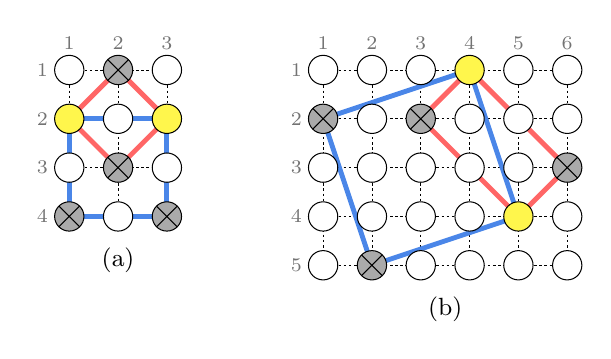
\begin{tikzpicture}[x=0.62cm,y=0.62cm,baseline=(current bounding box.north)]
  \begin{scope}[xshift=0.000cm]
    \draw[black,line width=0.25pt,dash pattern=on 0.93pt off 0.93pt] (1,-1) -- (3,-1) (1,-2) -- (3,-2) (1,-3) -- (3,-3) (1,-4) -- (3,-4) (1,-1) -- (1,-4) (2,-1) -- (2,-4) (3,-1) -- (3,-4);
    \draw[kblue,line width=1.76pt,line join=round] (1,-2) -- (3,-2) -- (3,-4) -- (1,-4) -- cycle;
    \draw[kred,line width=1.76pt,line join=round] (1,-2) -- (2,-1) -- (3,-2) -- (2,-3) -- cycle;
    \filldraw[fill=white,draw=black,line width=0.37pt] (1,-1) circle (0.3);
    \filldraw[fill=kgray,draw=black,line width=0.37pt] (2,-1) circle (0.3);
    \draw[black,line width=0.37pt] (1.788,-0.788) -- (2.212,-1.212) (1.788,-1.212) -- (2.212,-0.788);
    \filldraw[fill=white,draw=black,line width=0.37pt] (3,-1) circle (0.3);
    \filldraw[fill=kyellow,draw=black,line width=0.37pt] (1,-2) circle (0.3);
    \filldraw[fill=white,draw=black,line width=0.37pt] (2,-2) circle (0.3);
    \filldraw[fill=kyellow,draw=black,line width=0.37pt] (3,-2) circle (0.3);
    \filldraw[fill=white,draw=black,line width=0.37pt] (1,-3) circle (0.3);
    \filldraw[fill=kgray,draw=black,line width=0.37pt] (2,-3) circle (0.3);
    \draw[black,line width=0.37pt] (1.788,-2.788) -- (2.212,-3.212) (1.788,-3.212) -- (2.212,-2.788);
    \filldraw[fill=white,draw=black,line width=0.37pt] (3,-3) circle (0.3);
    \filldraw[fill=kgray,draw=black,line width=0.37pt] (1,-4) circle (0.3);
    \draw[black,line width=0.37pt] (0.788,-3.788) -- (1.212,-4.212) (0.788,-4.212) -- (1.212,-3.788);
    \filldraw[fill=white,draw=black,line width=0.37pt] (2,-4) circle (0.3);
    \filldraw[fill=kgray,draw=black,line width=0.37pt] (3,-4) circle (0.3);
    \draw[black,line width=0.37pt] (2.788,-3.788) -- (3.212,-4.212) (2.788,-4.212) -- (3.212,-3.788);
    \node[lab] at (1,-0.45) {1};
    \node[lab] at (2,-0.45) {2};
    \node[lab] at (3,-0.45) {3};
    \node[lab] at (0.45,-1) {1};
    \node[lab] at (0.45,-2) {2};
    \node[lab] at (0.45,-3) {3};
    \node[lab] at (0.45,-4) {4};
    \node[capt,anchor=north] at (2.00,-4.45) {(a)};
  \end{scope}
  \begin{scope}[xshift=3.224cm]
    \draw[black,line width=0.25pt,dash pattern=on 0.93pt off 0.93pt] (1,-1) -- (6,-1) (1,-2) -- (6,-2) (1,-3) -- (6,-3) (1,-4) -- (6,-4) (1,-5) -- (6,-5) (1,-1) -- (1,-5) (2,-1) -- (2,-5) (3,-1) -- (3,-5) (4,-1) -- (4,-5) (5,-1) -- (5,-5) (6,-1) -- (6,-5);
    \draw[kblue,line width=1.76pt,line join=round] (4,-1) -- (5,-4) -- (2,-5) -- (1,-2) -- cycle;
    \draw[kred,line width=1.76pt,line join=round] (4,-1) -- (6,-3) -- (5,-4) -- (3,-2) -- cycle;
    \filldraw[fill=white,draw=black,line width=0.37pt] (1,-1) circle (0.3);
    \filldraw[fill=white,draw=black,line width=0.37pt] (2,-1) circle (0.3);
    \filldraw[fill=white,draw=black,line width=0.37pt] (3,-1) circle (0.3);
    \filldraw[fill=kyellow,draw=black,line width=0.37pt] (4,-1) circle (0.3);
    \filldraw[fill=white,draw=black,line width=0.37pt] (5,-1) circle (0.3);
    \filldraw[fill=white,draw=black,line width=0.37pt] (6,-1) circle (0.3);
    \filldraw[fill=kgray,draw=black,line width=0.37pt] (1,-2) circle (0.3);
    \draw[black,line width=0.37pt] (0.788,-1.788) -- (1.212,-2.212) (0.788,-2.212) -- (1.212,-1.788);
    \filldraw[fill=white,draw=black,line width=0.37pt] (2,-2) circle (0.3);
    \filldraw[fill=kgray,draw=black,line width=0.37pt] (3,-2) circle (0.3);
    \draw[black,line width=0.37pt] (2.788,-1.788) -- (3.212,-2.212) (2.788,-2.212) -- (3.212,-1.788);
    \filldraw[fill=white,draw=black,line width=0.37pt] (4,-2) circle (0.3);
    \filldraw[fill=white,draw=black,line width=0.37pt] (5,-2) circle (0.3);
    \filldraw[fill=white,draw=black,line width=0.37pt] (6,-2) circle (0.3);
    \filldraw[fill=white,draw=black,line width=0.37pt] (1,-3) circle (0.3);
    \filldraw[fill=white,draw=black,line width=0.37pt] (2,-3) circle (0.3);
    \filldraw[fill=white,draw=black,line width=0.37pt] (3,-3) circle (0.3);
    \filldraw[fill=white,draw=black,line width=0.37pt] (4,-3) circle (0.3);
    \filldraw[fill=white,draw=black,line width=0.37pt] (5,-3) circle (0.3);
    \filldraw[fill=kgray,draw=black,line width=0.37pt] (6,-3) circle (0.3);
    \draw[black,line width=0.37pt] (5.788,-2.788) -- (6.212,-3.212) (5.788,-3.212) -- (6.212,-2.788);
    \filldraw[fill=white,draw=black,line width=0.37pt] (1,-4) circle (0.3);
    \filldraw[fill=white,draw=black,line width=0.37pt] (2,-4) circle (0.3);
    \filldraw[fill=white,draw=black,line width=0.37pt] (3,-4) circle (0.3);
    \filldraw[fill=white,draw=black,line width=0.37pt] (4,-4) circle (0.3);
    \filldraw[fill=kyellow,draw=black,line width=0.37pt] (5,-4) circle (0.3);
    \filldraw[fill=white,draw=black,line width=0.37pt] (6,-4) circle (0.3);
    \filldraw[fill=white,draw=black,line width=0.37pt] (1,-5) circle (0.3);
    \filldraw[fill=kgray,draw=black,line width=0.37pt] (2,-5) circle (0.3);
    \draw[black,line width=0.37pt] (1.788,-4.788) -- (2.212,-5.212) (1.788,-5.212) -- (2.212,-4.788);
    \filldraw[fill=white,draw=black,line width=0.37pt] (3,-5) circle (0.3);
    \filldraw[fill=white,draw=black,line width=0.37pt] (4,-5) circle (0.3);
    \filldraw[fill=white,draw=black,line width=0.37pt] (5,-5) circle (0.3);
    \filldraw[fill=white,draw=black,line width=0.37pt] (6,-5) circle (0.3);
    \node[lab] at (1,-0.45) {1};
    \node[lab] at (2,-0.45) {2};
    \node[lab] at (3,-0.45) {3};
    \node[lab] at (4,-0.45) {4};
    \node[lab] at (5,-0.45) {5};
    \node[lab] at (6,-0.45) {6};
    \node[lab] at (0.45,-1) {1};
    \node[lab] at (0.45,-2) {2};
    \node[lab] at (0.45,-3) {3};
    \node[lab] at (0.45,-4) {4};
    \node[lab] at (0.45,-5) {5};
    \node[capt,anchor=north] at (3.50,-5.45) {(b)};
  \end{scope}
\end{tikzpicture}

\caption{Two mixed pairs. The common corners $p,q$ are yellow, $R_1$ is blue, and $R_2$ is
red. If the 4 points of the support are black, then both rectangles show exactly $p$
and $q$.}
\label{fig:mixed}
\end{figure}

In a mixed pair the rectangles are not both axis-aligned, since a side of an axis-aligned
rectangle is horizontal or vertical and a diagonal is not. We record the equations of a
support.

\begin{lemma}\label{lem:mixedeq}
Let $A,B,C,D$ be the support of a mixed pair as in Definition~\ref{def:mixed}. Then there is
a nonzero integer vector $n$ such that
\[
 n\cdot(B-A)=0,\qquad C+D=A+B+2n,\qquad |D-C|=|B-A|,\qquad D-C\ne\pm(B-A).
\]
\end{lemma}

\begin{proof}
Name the common corners so that $p=A+n$ and $q=B+n$. Then $n$ is a nonzero integer vector
perpendicular to the side $AB$. The diagonals $pq$ and $CD$ of $R_2$ have the same midpoint
and the same length, which gives the next 2 equations. If $D-C=\pm(B-A)=\pm(q-p)$, then
$\{C,D\}=\{p,q\}$.
\end{proof}

\begin{lemma}[criterion]\label{lem:criterion}
Let $S$ be a blackout of the $h\times m$ grid. Suppose that
\begin{enumerate}[(i)]
\item the graph $G_S$ has no cycle of length $4$ or $6$,
\item no tilted rectangle has 3 or more black corners, and
\item no mixed pair has all 4 points of its support black.
\end{enumerate}
Then $S$ is valid.
\end{lemma}

\begin{proof}
Suppose that $R_1\ne R_2$ have the same presentation. By Lemma~\ref{lem:diff}, the set
$D=C(R_1)\triangle C(R_2)$ is black. By (i) and Lemma~\ref{lem:girth} below, whose proof
does not use this lemma, the rectangles are not both axis-aligned. By
Lemma~\ref{lem:threecorners} they have at most 2 common corners. With no common corner,
both rectangles are fully black. With 1 common corner, both have 3 black corners. One of
them is tilted, so both cases contradict (ii). Suppose finally that they have 2 common
corners $p$ and $q$. If $pq$ is a side of both or a diagonal of both, then $D$ is the
corner set of a rectangle $R_3$ by Lemma~\ref{lem:compress}, and $R_3$ is fully black. If
$R_3$ is tilted, this contradicts (ii). If $R_3$ is axis-aligned, its corners give a cycle
of length $4$ in $G_S$, which contradicts (i). Otherwise $(R_1,R_2)$ or $(R_2,R_1)$ is a
mixed pair with support $D$, which contradicts (iii).
\end{proof}

\section{The row bound and the equality structure}\label{sec:graph}

A blackout $S$ is \emph{axis-valid} if distinct axis-aligned rectangles have distinct
presentations. Recall that the row-column graph $G_S$ joins row $r_j$ to column $c_i$ for
each black point $(i,j)$.

\begin{lemma}\label{lem:girth}
If $G_S$ has no cycle of length $4$ or $6$, then $S$ is axis-valid. The converse holds for
$m\ge3$.
\end{lemma}

\begin{proof}
Let $R_1\ne R_2$ be axis-aligned with the same presentation, so that
$C(R_1)\triangle C(R_2)\subseteq S$. They cannot share opposite corners. Hence their common
corners lie in one row or in one column, and by symmetry we can assume that they lie in one
row $a$. With no common corner, $R_1$ is fully black, which gives a cycle of length $4$.
With 2 common corners $(x,a)$ and $(y,a)$, the other rows $b\ne c$ of $R_1$ and $R_2$ give
the cycle $r_b\,c_x\,r_c\,c_y$. With just 1 common corner $(x,a)$, write
$R_1=\{x,y\}\times\{a,b\}$ and $R_2=\{x,z\}\times\{a,c\}$. Then $y\ne z$ and $b\ne c$, and
the 6 black points give the cycle $r_a\,c_y\,r_b\,c_x\,r_c\,c_z$.

Conversely, let $m\ge3$. A cycle $r_j\,c_i\,r_{j'}\,c_{i'}$ gives the rectangles
$\{i,w\}\times\{j,j'\}$ and $\{i',w\}\times\{j,j'\}$ for a third column $w$, and both show
exactly their white corners in column $w$. A cycle $r_a\,c_x\,r_b\,c_y\,r_c\,c_z$ gives the
rectangles $\{x,y\}\times\{a,b\}$ and $\{y,z\}\times\{a,c\}$. Both are black except possibly
at $(y,a)$.
\end{proof}

\begin{theorem}[row bound]\label{thm:rowbound}
Let $m\ge3$. Every axis-valid blackout of the $h\times m$ grid has at most $m+q_h$ points.
Hence $f(h,m)\le m+q_h$.
\end{theorem}

In graph terms this is the bound of Neuwirth \cite[Theorem~1(ii) and
Proposition~17]{neuwirth2001} for bipartite graphs without cycles of length $4$ and $6$,
which he states for $m\ge q_h$. His proof contracts each column to the pairs of its black
rows. The contracted graph on the rows is triangle-free with at most $q_h$ edges, so at
most $q_h$ columns have 2 or more black points \cite[Proposition~3]{neuwirth2001}, and he
bounds the number of edges at these columns by his cubic inequality
\cite[Theorem~1(i)]{neuwirth2001}. He shows that the bound is attained, but he does not
describe all graphs that attain it. His Remark~18 gives the maximum for $h\le5$. It is
$m+h-1$ for $h\le3$, $m+4$ for $h=4\le m$, and $m+6$ for $h=5<m$. For example the maximum
for the graph is $8$ when $h=m=4$, while $f(4,4)=7$. We give a short proof by Mantel's
theorem~\cite{mantel1907} because we need its cases of equality. We join the black rows
$B_i$ of each nonempty column by a tree $T_i$, so that the graph on the rows stays
triangle-free when a column has 3 or more black rows. Let $H$ be the union of these trees,
a graph on the $h$ rows.

\begin{lemma}\label{lem:H}
Let $m\ge3$ and let $S$ be axis-valid. For any choice of the trees, $H$ is simple and
triangle-free, and $e(H)=|S|-t$, where $t$ is the number of nonempty columns.
\end{lemma}

\begin{proof}
By Lemma~\ref{lem:girth}, $G_S$ has no cycle of length $4$ or $6$. A repeated edge of $H$
would put the same row pair in 2 columns, which gives a cycle of length $4$. Hence
$e(H)=\sum_i(|B_i|-1)=|S|-t$. Suppose that $H$ contains a triangle $r_ar_br_c$. Its edges
do not all belong to one tree. If 2 columns $i,i'$ supply them, then 2 of $a,b,c$ belong to
$B_i\cap B_{i'}$, which again gives a cycle of length $4$. If 3 columns supply them, we get
the cycle $r_a\,c_i\,r_b\,c_{i'}\,r_c\,c_{i''}$ of length $6$.
\end{proof}

\begin{lemma}[Mantel]\label{lem:mantel}
Let $H$ be a simple triangle-free graph on $h$ vertices. Let a vertex of maximum degree
$\Delta$ have neighbor set $\Gamma$, and let $\Omega$ be the set of the other $h-\Delta$
vertices, which spans $e(\Omega)$ edges. Then
\[
e(H)=\sum_{b\in\Omega}d(b)-e(\Omega)\le(h-\Delta)\Delta-e(\Omega)\le q_h.
\]
\end{lemma}

\begin{proof}
The set $\Gamma$ is independent, so every edge meets $\Omega$. The degree sum over $\Omega$
counts the edges inside $\Omega$ twice. Then use $d(b)\le\Delta$ and
$(h-\Delta)\Delta\le q_h$.
\end{proof}

\begin{proof}[Proof of Theorem~\ref{thm:rowbound}]
Lemmas~\ref{lem:H} and~\ref{lem:mantel} give $|S|=t+e(H)\le m+q_h$.
\end{proof}

\begin{theorem}[equality structure]\label{thm:equality}
Let $h\ge4$ and $m\ge3$. A blackout of the $h\times m$ grid with $m+q_h$ points is
axis-valid if and only if
\begin{enumerate}[(a)]
\item every column is a singleton or a double,
\item the $q_h$ doubles have distinct row pairs, and
\item these pairs are the edges of a complete bipartite graph on the rows with parts of
sizes $\lfloor h/2\rfloor$ and $\lceil h/2\rceil$.
\end{enumerate}
\end{theorem}

\begin{proof}
Let $S$ be axis-valid with $m+q_h$ points. Equality in the proof of the row bound forces
$t=m$, $e(\Omega)=0$, $(h-\Delta)\Delta=q_h$, and $d(b)=\Delta$ for every $b\in\Omega$.
Thus $H$ is the complete bipartite graph between $\Gamma$ and $\Omega$, as in (c), for
every choice of the trees. Suppose that $|B_i|\ge3$. Then $T_i$ has a vertex $v$ with 2
neighbors $u$ and $w$, which lie in one part. Since $h\ge4$, the part of $v$ contains
another vertex $z$. Replace the edge $vw$ of $T_i$ by $uw$. This gives another tree on
$B_i$, and the new graph $H$ contains $uz$, $wz$, and $uw$, which contradicts
Lemma~\ref{lem:H}. This proves (a). The tree edges are now the row pairs of the doubles,
which gives (b) and (c).

Conversely, assume (a) to (c). By (a) and (b), no 2 columns share 2 black rows, so $G_S$
has no cycle of length $4$. A cycle $r_a\,c_x\,r_b\,c_y\,r_c\,c_z$ needs doubles on
$\{a,b\}$, $\{b,c\}$, and $\{a,c\}$, which contradicts (c). Now apply
Lemma~\ref{lem:girth}.
\end{proof}

The graph $G_S$ of such a blackout is the extremal graph of Neuwirth from the
introduction.

\begin{corollary}\label{cor:small-m}
Let $h\ge4$ and $3\le m<q_h$. Then $f(h,m)\le m+q_h-1$. Hence $m_h\ge q_h$ for $h\ge4$.
\end{corollary}

\begin{proof}
A valid blackout with $m+q_h$ points would have $q_h$ doubles in different columns by
Theorem~\ref{thm:equality}. For the last statement, note that $q_h-1\ge3$.
\end{proof}

This proves Theorem~\ref{thm:threshold}(a). We end the section with a lower bound that
holds on every grid.

\begin{lemma}[boundary cross]\label{lem:cross}
The first row and the first column of the $h\times m$ grid form a valid blackout. Hence
$f(h,m)\ge h+m-1$.
\end{lemma}

\begin{proof}
The graph $G_S$ is a tree, so (i) of Lemma~\ref{lem:criterion} holds. Let $R$ be a tilted
rectangle with corners~\eqref{eq:tilt-param}. By Lemma~\ref{lem:leftmost}, its only
possible corner in column $1$ is $\ell$, and its only possible corner in row $1$ is
$\ell+(a,-b)$. Hence (ii) holds, and 2 black corners of a tilted rectangle are always
adjacent. Let $(R_1,R_2)$ be a mixed pair with black support $A,B,C,D$. The corners $C,D$
of $R_2$ are black and opposite, so $R_2$ is axis-aligned and $R_1$ is tilted. Then
$\{A,B\}=\{\ell,\ell+(a,-b)\}$ with $\ell=(1,1+b)$, and the common corners
$p=(1+c,1+b+d)$ and $q=(1+a+c,1+d)$ lie in columns and rows at least $2$. The other
corners $C,D$ of the axis-aligned rectangle with diagonal $pq$ also lie in columns and rows
at least $2$, so they are white, a contradiction. Thus (iii) holds.
\end{proof}

\section{An explicit construction at every height}\label{sec:general}

We now prove Proposition~\ref{thm:general}. We place the doubles far apart and let the
singletons between them be black in a boundary row. Call a singleton a \emph{sea} if its
black point lies in row $1$ or in row $h$.

\begin{proposition}[alternating seas]\label{prop:seas}
Let $h\ge3$ and let $H$ be a triangle-free graph on the rows with edges $e_1,\dots,e_q$,
where $q\ge1$. Let $Z$ be the blackout of the $h\times m$ grid with the following columns.
The columns $p_1<\dots<p_q$ are doubles, where column $p_j$ is black exactly in the 2 rows
of $e_j$ and $p_{j+1}-p_j\ge W_h+1$. Every other column is a sea. The seas to the left of
$p_1$ are black in row $1$, and the row of the seas switches between $1$ and $h$ at every
double. Then $Z$ is valid and $|Z|=m+q$.
\end{proposition}

\begin{figure}[ht]
\centering
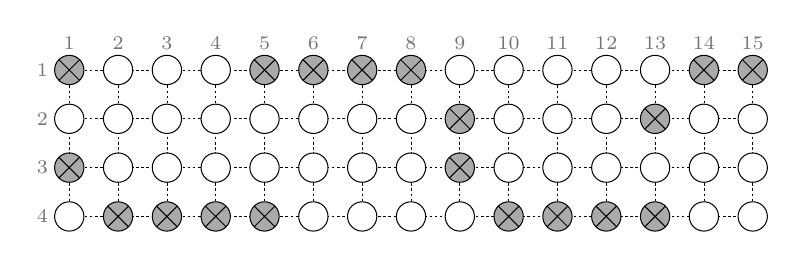
\begin{tikzpicture}[x=0.62cm,y=0.62cm,baseline=(current bounding box.north)]
  \begin{scope}[xshift=0.000cm]
    \draw[black,line width=0.25pt,dash pattern=on 0.93pt off 0.93pt] (1,-1) -- (15,-1) (1,-2) -- (15,-2) (1,-3) -- (15,-3) (1,-4) -- (15,-4) (1,-1) -- (1,-4) (2,-1) -- (2,-4) (3,-1) -- (3,-4) (4,-1) -- (4,-4) (5,-1) -- (5,-4) (6,-1) -- (6,-4) (7,-1) -- (7,-4) (8,-1) -- (8,-4) (9,-1) -- (9,-4) (10,-1) -- (10,-4) (11,-1) -- (11,-4) (12,-1) -- (12,-4) (13,-1) -- (13,-4) (14,-1) -- (14,-4) (15,-1) -- (15,-4);
    \filldraw[fill=kgray,draw=black,line width=0.37pt] (1,-1) circle (0.3);
    \draw[black,line width=0.37pt] (0.788,-0.788) -- (1.212,-1.212) (0.788,-1.212) -- (1.212,-0.788);
    \filldraw[fill=white,draw=black,line width=0.37pt] (2,-1) circle (0.3);
    \filldraw[fill=white,draw=black,line width=0.37pt] (3,-1) circle (0.3);
    \filldraw[fill=white,draw=black,line width=0.37pt] (4,-1) circle (0.3);
    \filldraw[fill=kgray,draw=black,line width=0.37pt] (5,-1) circle (0.3);
    \draw[black,line width=0.37pt] (4.788,-0.788) -- (5.212,-1.212) (4.788,-1.212) -- (5.212,-0.788);
    \filldraw[fill=kgray,draw=black,line width=0.37pt] (6,-1) circle (0.3);
    \draw[black,line width=0.37pt] (5.788,-0.788) -- (6.212,-1.212) (5.788,-1.212) -- (6.212,-0.788);
    \filldraw[fill=kgray,draw=black,line width=0.37pt] (7,-1) circle (0.3);
    \draw[black,line width=0.37pt] (6.788,-0.788) -- (7.212,-1.212) (6.788,-1.212) -- (7.212,-0.788);
    \filldraw[fill=kgray,draw=black,line width=0.37pt] (8,-1) circle (0.3);
    \draw[black,line width=0.37pt] (7.788,-0.788) -- (8.212,-1.212) (7.788,-1.212) -- (8.212,-0.788);
    \filldraw[fill=white,draw=black,line width=0.37pt] (9,-1) circle (0.3);
    \filldraw[fill=white,draw=black,line width=0.37pt] (10,-1) circle (0.3);
    \filldraw[fill=white,draw=black,line width=0.37pt] (11,-1) circle (0.3);
    \filldraw[fill=white,draw=black,line width=0.37pt] (12,-1) circle (0.3);
    \filldraw[fill=white,draw=black,line width=0.37pt] (13,-1) circle (0.3);
    \filldraw[fill=kgray,draw=black,line width=0.37pt] (14,-1) circle (0.3);
    \draw[black,line width=0.37pt] (13.788,-0.788) -- (14.212,-1.212) (13.788,-1.212) -- (14.212,-0.788);
    \filldraw[fill=kgray,draw=black,line width=0.37pt] (15,-1) circle (0.3);
    \draw[black,line width=0.37pt] (14.788,-0.788) -- (15.212,-1.212) (14.788,-1.212) -- (15.212,-0.788);
    \filldraw[fill=white,draw=black,line width=0.37pt] (1,-2) circle (0.3);
    \filldraw[fill=white,draw=black,line width=0.37pt] (2,-2) circle (0.3);
    \filldraw[fill=white,draw=black,line width=0.37pt] (3,-2) circle (0.3);
    \filldraw[fill=white,draw=black,line width=0.37pt] (4,-2) circle (0.3);
    \filldraw[fill=white,draw=black,line width=0.37pt] (5,-2) circle (0.3);
    \filldraw[fill=white,draw=black,line width=0.37pt] (6,-2) circle (0.3);
    \filldraw[fill=white,draw=black,line width=0.37pt] (7,-2) circle (0.3);
    \filldraw[fill=white,draw=black,line width=0.37pt] (8,-2) circle (0.3);
    \filldraw[fill=kgray,draw=black,line width=0.37pt] (9,-2) circle (0.3);
    \draw[black,line width=0.37pt] (8.788,-1.788) -- (9.212,-2.212) (8.788,-2.212) -- (9.212,-1.788);
    \filldraw[fill=white,draw=black,line width=0.37pt] (10,-2) circle (0.3);
    \filldraw[fill=white,draw=black,line width=0.37pt] (11,-2) circle (0.3);
    \filldraw[fill=white,draw=black,line width=0.37pt] (12,-2) circle (0.3);
    \filldraw[fill=kgray,draw=black,line width=0.37pt] (13,-2) circle (0.3);
    \draw[black,line width=0.37pt] (12.788,-1.788) -- (13.212,-2.212) (12.788,-2.212) -- (13.212,-1.788);
    \filldraw[fill=white,draw=black,line width=0.37pt] (14,-2) circle (0.3);
    \filldraw[fill=white,draw=black,line width=0.37pt] (15,-2) circle (0.3);
    \filldraw[fill=kgray,draw=black,line width=0.37pt] (1,-3) circle (0.3);
    \draw[black,line width=0.37pt] (0.788,-2.788) -- (1.212,-3.212) (0.788,-3.212) -- (1.212,-2.788);
    \filldraw[fill=white,draw=black,line width=0.37pt] (2,-3) circle (0.3);
    \filldraw[fill=white,draw=black,line width=0.37pt] (3,-3) circle (0.3);
    \filldraw[fill=white,draw=black,line width=0.37pt] (4,-3) circle (0.3);
    \filldraw[fill=white,draw=black,line width=0.37pt] (5,-3) circle (0.3);
    \filldraw[fill=white,draw=black,line width=0.37pt] (6,-3) circle (0.3);
    \filldraw[fill=white,draw=black,line width=0.37pt] (7,-3) circle (0.3);
    \filldraw[fill=white,draw=black,line width=0.37pt] (8,-3) circle (0.3);
    \filldraw[fill=kgray,draw=black,line width=0.37pt] (9,-3) circle (0.3);
    \draw[black,line width=0.37pt] (8.788,-2.788) -- (9.212,-3.212) (8.788,-3.212) -- (9.212,-2.788);
    \filldraw[fill=white,draw=black,line width=0.37pt] (10,-3) circle (0.3);
    \filldraw[fill=white,draw=black,line width=0.37pt] (11,-3) circle (0.3);
    \filldraw[fill=white,draw=black,line width=0.37pt] (12,-3) circle (0.3);
    \filldraw[fill=white,draw=black,line width=0.37pt] (13,-3) circle (0.3);
    \filldraw[fill=white,draw=black,line width=0.37pt] (14,-3) circle (0.3);
    \filldraw[fill=white,draw=black,line width=0.37pt] (15,-3) circle (0.3);
    \filldraw[fill=white,draw=black,line width=0.37pt] (1,-4) circle (0.3);
    \filldraw[fill=kgray,draw=black,line width=0.37pt] (2,-4) circle (0.3);
    \draw[black,line width=0.37pt] (1.788,-3.788) -- (2.212,-4.212) (1.788,-4.212) -- (2.212,-3.788);
    \filldraw[fill=kgray,draw=black,line width=0.37pt] (3,-4) circle (0.3);
    \draw[black,line width=0.37pt] (2.788,-3.788) -- (3.212,-4.212) (2.788,-4.212) -- (3.212,-3.788);
    \filldraw[fill=kgray,draw=black,line width=0.37pt] (4,-4) circle (0.3);
    \draw[black,line width=0.37pt] (3.788,-3.788) -- (4.212,-4.212) (3.788,-4.212) -- (4.212,-3.788);
    \filldraw[fill=kgray,draw=black,line width=0.37pt] (5,-4) circle (0.3);
    \draw[black,line width=0.37pt] (4.788,-3.788) -- (5.212,-4.212) (4.788,-4.212) -- (5.212,-3.788);
    \filldraw[fill=white,draw=black,line width=0.37pt] (6,-4) circle (0.3);
    \filldraw[fill=white,draw=black,line width=0.37pt] (7,-4) circle (0.3);
    \filldraw[fill=white,draw=black,line width=0.37pt] (8,-4) circle (0.3);
    \filldraw[fill=white,draw=black,line width=0.37pt] (9,-4) circle (0.3);
    \filldraw[fill=kgray,draw=black,line width=0.37pt] (10,-4) circle (0.3);
    \draw[black,line width=0.37pt] (9.788,-3.788) -- (10.212,-4.212) (9.788,-4.212) -- (10.212,-3.788);
    \filldraw[fill=kgray,draw=black,line width=0.37pt] (11,-4) circle (0.3);
    \draw[black,line width=0.37pt] (10.788,-3.788) -- (11.212,-4.212) (10.788,-4.212) -- (11.212,-3.788);
    \filldraw[fill=kgray,draw=black,line width=0.37pt] (12,-4) circle (0.3);
    \draw[black,line width=0.37pt] (11.788,-3.788) -- (12.212,-4.212) (11.788,-4.212) -- (12.212,-3.788);
    \filldraw[fill=kgray,draw=black,line width=0.37pt] (13,-4) circle (0.3);
    \draw[black,line width=0.37pt] (12.788,-3.788) -- (13.212,-4.212) (12.788,-4.212) -- (13.212,-3.788);
    \filldraw[fill=white,draw=black,line width=0.37pt] (14,-4) circle (0.3);
    \filldraw[fill=white,draw=black,line width=0.37pt] (15,-4) circle (0.3);
    \node[lab] at (1,-0.45) {1};
    \node[lab] at (2,-0.45) {2};
    \node[lab] at (3,-0.45) {3};
    \node[lab] at (4,-0.45) {4};
    \node[lab] at (5,-0.45) {5};
    \node[lab] at (6,-0.45) {6};
    \node[lab] at (7,-0.45) {7};
    \node[lab] at (8,-0.45) {8};
    \node[lab] at (9,-0.45) {9};
    \node[lab] at (10,-0.45) {10};
    \node[lab] at (11,-0.45) {11};
    \node[lab] at (12,-0.45) {12};
    \node[lab] at (13,-0.45) {13};
    \node[lab] at (14,-0.45) {14};
    \node[lab] at (15,-0.45) {15};
    \node[lab] at (0.45,-1) {1};
    \node[lab] at (0.45,-2) {2};
    \node[lab] at (0.45,-3) {3};
    \node[lab] at (0.45,-4) {4};
  \end{scope}
\end{tikzpicture}

\caption{The blackout of Proposition~\ref{prop:seas} for $h=4$ and $m=15$, with the 4 edges
of the complete bipartite graph between $\{1,2\}$ and $\{3,4\}$. Here $W_4+1=4$.}
\label{fig:seas}
\end{figure}

\begin{proof}[Proof of Proposition~\ref{thm:general}]
Theorem~\ref{thm:rowbound} gives the upper bound. Take $H$ to be the complete bipartite
graph with parts of sizes $\lfloor h/2\rfloor$ and $\lceil h/2\rceil$, so $q=q_h$, and
place the doubles at $p_j=1+(j-1)(W_h+1)$. The last double is in column
$1+(q_h-1)(W_h+1)=M_h$. Hence Proposition~\ref{prop:seas} gives a valid blackout with
$m+q_h$ points for every $m\ge M_h$.
\end{proof}

\begin{proof}[Proof of Proposition~\ref{prop:seas}]
Each double adds 1 point to a column, so $|Z|=m+q$. We check the 3 conditions of
Lemma~\ref{lem:criterion}.

\emph{Condition (i).} Only doubles have 2 black rows, and their pairs are distinct, so
$G_Z$ has no cycle of length $4$. A cycle $r_a\,c_x\,r_b\,c_y\,r_c\,c_z$ would need doubles
on $\{a,b\}$, $\{b,c\}$, and $\{a,c\}$, a triangle in $H$.

\emph{The black corners of a tilted rectangle.} Let $R$ be a tilted rectangle. In this
proof, \emph{the columns of $R$} are all columns from its smallest to its largest column,
not only the columns of its corners. The span of $R$ is at most $W_h$
(Lemma~\ref{lem:span}), so its columns contain at most 1 double. With no
double, all black points in the columns of $R$ lie in one boundary row, and $R$ has at most
1 black corner by (F1). Otherwise, shift the double to column $0$ and write its black rows as
$a<b$. Reflecting the rows if needed, we can assume that the seas in the columns of $R$ are
black in row $1$ to the left of column $0$ and in row $h$ to the right.

Let $K$ be the set of black corners of $R$. By (F1), the elements of $K$ can only be one
point $u=(x_1,1)$ with $x_1<0$, one point $v=(x_2,h)$ with $x_2>0$, and points $(0,c)$ with
$c\in\{a,b\}$. A corner $(0,1)$ excludes $u$, and a corner $(0,h)$ excludes $v$. We now
list the sets $K$ with $|K|\ge2$. In each case we find the other corners of $R$.
\begin{enumerate}[(a)]
\item $K=\{u,v\}$. These corners are opposite by (F2). The other diagonal has midpoint
$\bigl(\frac{x_1+x_2}2,\frac{1+h}2\bigr)$ and endpoints at this midpoint plus and minus a
vector $w$ with $|w|^2=\frac14\bigl((x_2-x_1)^2+(h-1)^2\bigr)$. By (F1) the endpoints lie in
rows $2$ to $h-1$. Hence $|w_2|\le\frac{h-3}2$ and $w_1^2>\frac14(x_2-x_1)^2$. So one
endpoint lies to the left of column $x_1$ and the other to the right of column $x_2$.
\item $K=\{(0,a),(0,b)\}$. These corners are opposite by (F3). The other diagonal has
midpoint $\bigl(0,\frac{a+b}2\bigr)$ and length $b-a$, and it is not vertical. Hence its
endpoints lie in columns $-w_1$ and $w_1$ for some $w_1\ne0$, and in rows strictly between
$a$ and $b$.
\item $K=\{u,d\}$ with $d=(0,c)$, and $u,d$ are opposite. Here $c\ge2$ by (F1). The other
diagonal has midpoint $\bigl(\frac{x_1}2,\frac{1+c}2\bigr)$ and endpoints at this midpoint
plus and minus a vector $w$ with $|w|^2=\frac14\bigl(x_1^2+(c-1)^2\bigr)$. The endpoints
are not in row $1$ by (F1). They are not in row $h$ by (F2), since the corner opposite to
$u$ is $d$. They are not in column $0$ by (F3), for the same reason. Since their rows are
at least $2$, we get $|w_2|\le\frac{c-3}2$. In particular $c\ge3$, and
$w_1^2>\frac14x_1^2$. Thus one endpoint
lies to the right of column $0$ and the other to the left of column $x_1$.
\item $K=\{u,d\}$ with $d=(0,c)$, and $u,d$ are adjacent. Again $c\ge2$. The side $d-u$ is
$(|x_1|,c-1)$, and the other corners are $u+n$ and $d+n$ with $n=t\,(-(c-1),|x_1|)$ for
some real $t\ne0$. The corner $u+n$ lies in row $1+t|x_1|$, so $t>0$. Hence both corners lie in
columns to the left of column $0$ and in rows at least $2$.
\item $K=\{v,d\}$ with $d=(0,c)$. The half turn $(x,j)\mapsto(-x,h+1-j)$ exchanges the 2
seas and fixes column $0$. It reduces this case to (c) or (d).
\item $|K|\ge3$. This is impossible. If $K$ contains $(0,a)$ and $(0,b)$, then the other 2
corners lie in rows strictly between $a$ and $b$ by (b), so they are neither $u$ nor $v$,
and they are not in column $0$. Otherwise $K=\{u,d,v\}$ with $d=(0,c)$. Then $u$ and $v$
are opposite by (F2) and $d$ is adjacent to both. So $(u-d)\cdot(v-d)=0$, that is
$x_1x_2=(c-1)(h-c)$. The left side is negative and the right side is not.
\end{enumerate}
In (a) to (d), the 2 other corners lie in columns different from $0$ and in rows $2$ to
$h-1$, or to the left of column $0$ and in rows at least $2$. The seas in these columns are
black only in row $1$ or only in row $h$, so the 2 other corners are white. By (e) the same
holds in the reflected cases. We have proved the following 3 statements for a tilted
rectangle $R$.
\begin{enumerate}[(1)]
\item $R$ has at most 2 black corners. Hence condition (ii) holds.
\item If $R$ has 2 opposite black corners, then its 2 white corners lie in rows $2$ to $h-1$,
one of them to the left and the other to the right of the double in the columns of $R$.
\item If $R$ has 2 adjacent black corners, then both white corners of $R$ lie on one side
of the double in the columns of $R$. On this side the seas in the columns of $R$ are black
in one boundary row, and the white corners are not in that row.
\end{enumerate}

\emph{Condition (iii).} Let $(R_1,R_2)$ be a mixed pair with common corners $p,q$ whose
support is black. A tilted rectangle of the pair has 2 black corners in the support, so its
corners $p,q$ are white by (1).

Suppose that $R_1$ is axis-aligned. Then $R_2$ is tilted with 2 opposite black corners. By
(2), $p$ and $q$ lie in different columns $x<z$ on the 2 sides of the double of $R_2$. So
the side $pq$ of $R_1$ is horizontal. The other 2 corners of $R_1$ are black points of the
columns $x$ and $z$ in a common row. But these columns are seas, one black only in row $1$
and the other only in row $h$, a contradiction.

Suppose that $R_2$ is axis-aligned. Then $R_1$ is tilted with 2 adjacent black corners. By
(3), $p=(x,j)$ and $q=(z,k)$ lie in sea columns that are black only in one boundary row
$\sigma$, and $j,k\ne\sigma$. The other corners of $R_2$ are $(x,k)$ and $(z,j)$, which are
white, a contradiction.

Suppose finally that both are tilted. The side opposite to $pq$ in $R_1$ is black, so (3)
applies to $R_1$. Let $D_1$ be the column of the double in the columns of $R_1$. Then $p$
and $q$ lie on one side of column $D_1$. The diagonal of $R_2$ other than $pq$ is black, so
(2) applies to $R_2$. Let $D_2$ be the column of the double in the columns of $R_2$. Then
$D_2$ lies strictly between the columns of $p$ and $q$. Hence $D_2\ne D_1$, and $D_2$ is a
second double in the columns of $R_1$, a contradiction. Thus (iii) holds, and $Z$ is valid by
Lemma~\ref{lem:criterion}.
\end{proof}

\begin{remark}\label{rem:spacing}
The proof uses the spacing $W_h+1$ only to keep 2 doubles out of the columns of one tilted
rectangle. The spacing $W_h$ is not always enough. Take the complete bipartite graph
between the rows $1,\dots,\lfloor h/2\rfloor$ and the other rows, with the doubles in
lexicographic order of their row pairs. Then the blackout with spacing $W_h$ is valid for
$h=3,5,7$ and not valid for $h=4,6,8$.
\end{remark}

\section{The threshold is nearly quadratic}\label{sec:threshold}

In this section we prove Theorem~\ref{thm:threshold}(b). A \emph{parity edge} is a pair
$\{r,s\}$ of rows with $r$ odd and $s$ even. There are $q_h$ parity edges, and they are the
edges of a complete bipartite graph as in Theorem~\ref{thm:equality}(c). Our blackouts have
one double for each parity edge and a singleton in every other column. All singletons of a
long block of columns are black in one of 2 fixed rows, which we call the \emph{sea rows}.

\subsection{Obstructions}

It is convenient to work in the strip $\strip=\ZZ\times\{1,\dots,h\}$. A rectangle
\emph{of the strip} has its corners in $\strip$. The lemmas of Section~\ref{sec:prelim} hold
in the strip with the same proofs. A \emph{configuration} is a subset of $\strip$, whose
points we call black.

\begin{definition}\label{def:obstruction}
We use 3 kinds of \emph{obstructions}.
\begin{enumerate}[(1)]
\item A \emph{corner triple} consists of 3 corners of a tilted rectangle of the strip.
\item A \emph{mixed quadruple} is the support $\{A,B,C,D\}$ of a mixed pair of the strip
whose side $AB$ is not vertical.
\item Let $R$ be a tilted rectangle of the strip that has a vertical diagonal $pq$, where
the rows of $p$ and $q$ have different parity. The other 2 corners of $R$ form a
\emph{rival pair}.
\end{enumerate}
A configuration \emph{contains} an obstruction if all points of the obstruction are black.
\end{definition}

The points of an obstruction always lie in $2W_h+1$ consecutive columns. For corner triples
and rival pairs this holds because a tilted rectangle has span at most $W_h$. In a mixed
pair $(R_1,R_2)$ with common corners $p,q$, at least one rectangle is tilted. If both are
tilted, they share the corner $p$ and have span at most $W_h$. If $R_2$ is axis-aligned,
its columns are those of $p$ and $q$, which are columns of $R_1$. If $R_1$ is axis-aligned
and $pq$ is not vertical, then $pq$ is horizontal, and the columns of $R_1$ are again those
of $p$ and $q$. A mixed pair with a vertical side $pq$ does not give a mixed quadruple. It
gives a rival pair (Lemma~\ref{lem:reduction}).

\begin{lemma}[reduction]\label{lem:reduction}
Let $S$ be a blackout of the $h\times m$ grid. Suppose that every column is a singleton or a
double, that the doubles have distinct row pairs, and that these pairs are parity edges. If
$S$ contains no obstruction, then $S$ is valid.
\end{lemma}

\begin{proof}
We check the conditions of Lemma~\ref{lem:criterion}. The graph $G_S$ has no cycle of length
$4$ because the doubles have distinct pairs. A cycle of length $6$ would need 3 doubles
whose pairs form a triangle, but the parity edges form a bipartite graph. A tilted
rectangle with 3 black corners gives a corner triple. Let $(R_1,R_2)$ be a mixed pair with
common corners $p,q$ and black support $A,B,C,D$. If the side $AB$ is not vertical, the
support is a mixed quadruple. Suppose that $AB$ is vertical. Then $A$ and $B$ are 2 black
points of one column, so their rows form a parity edge. The side $pq$ of $R_1$ is vertical
with the same 2 rows. Now $pq$ is a diagonal of $R_2$, so $R_2$ is tilted, and $\{C,D\}$ is
a rival pair.
\end{proof}

The next 3 lemmas show that some simple configurations contain no obstructions.

\begin{lemma}[rival pairs]\label{lem:rival}
Let $\{C,D\}$ be a rival pair with $C$ in row $c$, $D$ in row $c'$, and $c\le c'$. Then
$c'-c$ is odd, and there is an integer $j\ge1$ with
\[
 c-j\ge1,\qquad c'+j\le h,\qquad 4j(c'-c+j)=(C_x-D_x)^2 ,
\]
where $C_x$ and $D_x$ are the columns of $C$ and $D$. In particular, no point of a rival
pair lies in row $1$ or in row $h$, and the 2 points lie in rows of different parity.
\end{lemma}

\begin{proof}
Let $R$ and $pq$ be as in Definition~\ref{def:obstruction}(3), and let $L$ be the length of
$pq$. Then $L$ is an odd integer. The diagonals $pq$ and $CD$ have the same midpoint and the
same length. Put $t=C_x-D_x$ and $d=c'-c$, so that $L^2=t^2+d^2$. Here $t\ne0$, since $CD$
is not vertical, and so $L>d$. The rows of $p$ and $q$ are $\frac12(c+c'-L)$ and
$\frac12(c+c'+L)$. They are integers, so $L-d$ is even. Write $L=d+2j$ with $j\ge1$. Then
$d$ is odd, the rows of $p$ and $q$ are $c-j$ and $c'+j$, and
$t^2=L^2-d^2=4j(d+j)$.
\end{proof}

\begin{lemma}[two sea rows]\label{lem:sea}
Let $g$ be an even integer with $2\le g\le h$ and $2g-1>h$. No obstruction has all its
points in the rows $1$ and $g$.
\end{lemma}

\begin{proof}
Suppose that 3 corners of a tilted rectangle $R$ lie in the rows $1$ and $g$. Then 2 of
them lie in one row $y_0$, and they are opposite by (F3). So no other corner lies in row
$y_0$, and the third corner lies in the other row $y_1$. The center of $R$ is in row $y_0$, so the fourth corner is in row
$2y_0-y_1$. This row is $2-g<1$ or $2g-1>h$, a contradiction.

Let $\{A,B,C,D\}$ be a mixed quadruple in the rows $1$ and $g$, and let $n=(n_1,n_2)$ be as
in Lemma~\ref{lem:mixedeq}. Write $B-A=(x,y)$, where $x\ne0$. The equation $C+D=A+B+2n$
shows that the rows of $C$ and $D$ have the same sum modulo $2$ as the rows of $A$ and
$B$. Since $1+g$ is odd, either both pairs lie in one row each, or both pairs meet both
rows. In the first case $y=0$, so $n_1x=0$ gives $n_1=0$, and $D-C$ is horizontal with
$|D-C|=|x|$. Then $D-C=\pm(B-A)$, a contradiction. In the second case the row sums are
equal, so $n_2=0$. Then $n_1x=0$ gives $n=0$, a contradiction.

By Lemma~\ref{lem:rival}, a rival pair has no point in row $1$ and does not lie in one row.
\end{proof}

A \emph{chain} is a set of points of $\ZZ^2$ in which any 2 points $P,P'$ satisfy $P\le P'$
or $P'\le P$ in both coordinates.

\begin{lemma}[chains]\label{lem:chain}
A chain contains no corner triple and no mixed quadruple.
\end{lemma}

\begin{proof}
Let $Q_0,Q_1,Q_2$ be a corner triple with the right angle at $Q_0$. The vectors $Q_1-Q_0$
and $Q_2-Q_0$ are sides of a tilted rectangle, so all their coordinates are nonzero. In a
chain, each of them has 2 positive or 2 negative coordinates. Then their dot product is not
$0$, a contradiction.

Let $\{A,B,C,D\}$ be a mixed quadruple in a chain, with $n$ as in
Lemma~\ref{lem:mixedeq}. We can name the points so that $A\le B$ and $C\le D$. Put
$U=B-A$ and $\varphi(P)=(P-A)\cdot U$. Then $\varphi(A)=0$ and $\varphi(B)=|U|^2$. The
equations $C+D=A+B+2n$ and $n\cdot U=0$ give $\varphi(C)+\varphi(D)=|U|^2$. Also
$|\varphi(D)-\varphi(C)|=|(D-C)\cdot U|<|U|^2$, because $|D-C|=|U|$ and $D-C\ne\pm U$.
Hence $0<\varphi(P)<|U|^2$ for $P\in\{C,D\}$. The coordinates of $U$ are nonnegative. So a
point $P\le A$ has $\varphi(P)\le0$, and a point $P\ge B$ has $\varphi(P)\ge|U|^2$. Since
the 4 points form a chain, we get $A\le C\le D\le B$. Then $0\le D-C\le B-A$ in both
coordinates, and $|D-C|=|B-A|$ forces $D-C=B-A$, a contradiction.
\end{proof}

Finally we count obstructions with given rows. Recall that
$\tmax(h)=\max\{\tau(n):1\le n\le h^2\}$.

\begin{lemma}[counting]\label{lem:count}
Fix rows $y_0,y_1,y_2,y_3$.
\begin{enumerate}[(a)]
\item There are at most $2\tmax(h)$ triples $(Q_0,Q_1,Q_2)$ such that $\{Q_0,Q_1,Q_2\}$ is a
corner triple with the right angle at $Q_0$, the point $Q_i$ lies in row $y_i$, and $Q_0$
lies in column $0$.
\item There are at most $4\tmax(h)$ quadruples $(A,B,C,D)$ that form a mixed quadruple with
side $AB$ and diagonal $CD$, with these points in the rows $y_0,y_1,y_2,y_3$ and with $A$
in column $0$.
\item There are at most $2\tmax(h)$ rival pairs $\{C,D\}$ with $C=(0,y_0)$ and $D$ in row
$y_1$.
\end{enumerate}
\end{lemma}

\begin{proof}
(a) Write $Q_1-Q_0=(x_1,y_1-y_0)$ and $Q_2-Q_0=(x_2,y_2-y_0)$. All 4 coordinates are
nonzero, and $x_1x_2=-(y_1-y_0)(y_2-y_0)$. So $x_1$ is a positive or negative divisor of a
fixed integer $k$ with $1\le|k|\le h^2$, and $x_1$ determines $x_2$.

(b) Let $n=(n_1,n_2)$ be as in Lemma~\ref{lem:mixedeq}, and write $B-A=(x,y)$ and
$D-C=(z,v)$. The rows fix $y$, $v$, and $n_2$, and we have $x\ne0$, $n_1x=-n_2y$, and
$x^2+y^2=z^2+v^2$. Suppose first that $y\ne0$. Then $n_2\ne0$, since otherwise $n=0$. So $x$
is a divisor of the integer $n_2y$, where $1\le|n_2y|\le h^2$. There are at most
$2\tmax(h)$ such $x$. Each of them determines $n_1$ and allows at most 2 values of $z$.
Suppose now that $y=0$. Then $n_1=0$ and $x^2-z^2=v^2$. Here $v\ne0$, since otherwise
$D-C=\pm(B-A)$. Hence $|x|-|z|$ is a divisor of $v^2$, and it determines $|x|$ and $|z|$.
This gives at most $4\tau(v^2)\le4\tmax(h)$ pairs $(x,z)$. In both cases $x$, $z$, and $n$
determine $B=A+(x,y)$ and then $C$ and $D$, by $C+D=A+B+2n$.

(c) By Lemma~\ref{lem:rival}, the column $t$ of $D$ satisfies $t^2+d^2=L^2$ with
$d=|y_1-y_0|\ge1$ and an integer $L$. Then $L-|t|$ is a divisor of $d^2$, and it
determines $|t|$.
\end{proof}

\subsection{One double}

Fix an even integer $g$ with $2\le g\le h$ and $2g-1>h$. The sea rows are $1$ and $g$.

\begin{definition}\label{def:good}
A parity edge $e=\{r,s\}$ with $r$ odd is \emph{good for $g$} if $r\le g$, $s\le g$, and
$j(g-r+j)$ is not a perfect square for any integer $j$ with $1\le j\le\min(r-1,h-g)$. Its
\emph{gadget} is the configuration
\[
 G_e=\{(x,1):x<0\}\cup\{(0,r),(0,s)\}\cup\{(x,g):x>0\}.
\]
An obstruction is \emph{private to $e$} if it has a point in column $0$, all its points
in column $0$ lie in the rows $r$ and $s$, and all its other points lie in the rows $1$ and
$g$. Let $A_e$ be the set of integers $a\ne0$ such that some corner triple or mixed
quadruple private to $e$ has a point in column $a$.
\end{definition}

The set $A_e$ lists the columns near a double on $e$ whose singletons can take part in a
confusion with this double alone. We will fix the singletons in these columns as in the
gadget.

\begin{lemma}[one double]\label{lem:onedouble}
Let $e$ be good for $g$.
\begin{enumerate}[(a)]
\item We have $|A_e|\le2^{14}\,\tmax(h)$, and $|a|\le2W_h$ for every $a\in A_e$.
\item The gadget $G_e$ contains no corner triple and no mixed quadruple.
\item No rival pair consists of a point $(0,c)$ with $c\in e$ and a point in row $1$ or
$g$.
\end{enumerate}
\end{lemma}

\begin{proof}
(a) In a private obstruction every point lies in one of the 4 rows $r,s,1,g$. By
Lemma~\ref{lem:count}(a), there are at most $4^3\cdot2\tmax(h)$ corner triples with rows
in this set, up to horizontal translations. Each of them has at most 3 translates with a
point in column $0$, and each translate has at most 2 other columns. This gives at most
$768\,\tmax(h)$ elements of $A_e$. In the same way, Lemma~\ref{lem:count}(b) gives at most
$4^4\cdot4\tmax(h)\cdot4\cdot3=12288\,\tmax(h)$ elements. The bound on $|a|$ holds because
an obstruction lies in $2W_h+1$ consecutive columns.

(b) Since $r,s\le g$, the gadget is a chain. Apply Lemma~\ref{lem:chain}.

(c) Let $\{(0,c),D\}$ be such a rival pair. By Lemma~\ref{lem:rival}, $D$ is not in row
$1$. So $D$ is in row $g$, and $c$ is odd, that is $c=r<g$. Lemma~\ref{lem:rival} gives
an integer $j$ with $1\le j\le\min(r-1,h-g)$ such that $4j(g-r+j)$ is a perfect square.
Then $j(g-r+j)$ is a perfect square, which contradicts Definition~\ref{def:good}.
\end{proof}

\subsection{Many doubles}

Let $\mathcal E$ be a set of parity edges that are good for $g$. We give each
$e\in\mathcal E$ a column $X_e$, and we put $A_e^*=A_e\cup\{0\}$. For a set
$L\subseteq\mathcal E$ with $2\le|L|\le4$, we say that the columns $(X_e)_{e\in L}$ are
\emph{bad} if at least one of the following holds.
\begin{enumerate}[(B1)]
\item $L=\{e,f\}$ and the sets $X_e+A_e^*$ and $X_f+A_f^*$ intersect.
\item $L=\{e,f\}$ and $\{(X_e,c),(X_f,c')\}$ is a rival pair for some $c\in e$ and
$c'\in f$.
\item The columns $X_e$ with $e\in L$ are distinct, and there is a corner triple or a
mixed quadruple $Q$ with the following 2 properties. Every point of $Q$ in a column $X_e$
with $e\in L$ lies in a row of $e$, and every other point of $Q$ lies in row $1$ or $g$.
For every $e\in L$, at least one point of $Q$ lies in column $X_e$.
\end{enumerate}

\begin{lemma}[placement]\label{lem:placement}
There is an absolute constant $c_0$ with the following property. Let $\mathcal E$ be a
set of $n\ge1$ parity edges that are good for $g$, and let $N\ge c_0\,n\,\tmax(h)^2$ be
an integer. Then there are columns $X_e\in\{1,\dots,N\}$ for $e\in\mathcal E$ such that
$(X_e)_{e\in L}$ is not bad for any $L\subseteq\mathcal E$ with $2\le|L|\le4$.
\end{lemma}

\begin{proof}
Choose the $X_e$ independently and uniformly from $\{1,\dots,N\}$, and let $E_L$ be the
event that $(X_e)_{e\in L}$ is bad. Write $\tmax=\tmax(h)$.

We first bound $\Pr(E_L)$. Fix one edge $e_0\in L$. Each of the conditions below fixes the
differences $X_e-X_{e_0}$ for all $e\in L$, so it holds with probability at most
$N^{-(|L|-1)}$. For (B1) there are at most $(|A_e|+1)(|A_f|+1)\le2^{30}\tmax^2$ possible
differences $X_f-X_e$, by Lemma~\ref{lem:onedouble}(a). For (B2) there are 4 choices of
$(c,c')$. By Lemma~\ref{lem:count}(c), the pair $\{(X_e,c),(X_f,c')\}$ is a rival pair only
if $X_f-X_e$ is one of at most $2\tmax$ integers.

For (B3), let $Q$ be as in (B3). If $Q$ is a corner triple, list its points as
$(Q_0,Q_1,Q_2)$ with the right angle at $Q_0$. If $Q$ is a mixed quadruple, list them as
$(A,B,C,D)$ with the side $AB$ and the diagonal $CD$. Give each point of the list a
\emph{type}. A point in a column $X_e$ with $e\in L$ gets the type $(e,c)$, where $c\in e$
is its row. This is well defined because the columns $X_e$ are distinct. Every other point
gets its row, which is $1$ or $g$, as its type. There are at most 10 types, so there are at
most $10^3+10^4$ lists of types, and every $e\in L$ occurs in the list of $Q$. Now fix a
list of types in which every $e\in L$ occurs. It fixes the rows of the points. By
Lemma~\ref{lem:count}(a) and (b), at most $4\tmax$ lists of points $Q^*$ of the same kind
have these rows and their first point in column $0$, and $Q$ is a horizontal translate of
one of them. Fix $Q^*$ as well. If $Q$ is the translate of $Q^*$ by $x$ columns, then $X_e$
is $x$ plus the column of every point of $Q^*$ of type $(e,c)$. Hence $Q^*$ and the list of
types determine all differences $X_e-X_{e_0}$ with $e\in L$. Altogether
we get $\Pr(E_L)\le p_{|L|}$, where
\[
 p_2=c_1\,\tmax^2N^{-1},\qquad p_3=c_1\,\tmax N^{-2},\qquad p_4=c_1\,\tmax N^{-3},
 \qquad c_1=2^{31}.
\]

The event $E_L$ depends only on the variables $X_e$ with $e\in L$. Hence $E_L$ is mutually
independent of the family of all events $E_{L'}$ with $L'\cap L=\emptyset$. We apply the
local lemma in its general form~\cite[Lemma~5.1.1]{alonspencer2016} with the weights
$x_L=2p_{|L|}$. Put $c_0=48c_1$. An edge $e$ lies in at most $n^{k-1}$ sets $L$ of size $k$.
For $N\ge c_0n\tmax^2$ this gives
\[
 \sum_{L\ni e}x_L\le2c_1\Bigl(\frac{n\tmax^2}{N}+\frac{n^2\tmax}{N^2}
 +\frac{n^3\tmax}{N^3}\Bigr)\le\frac{6c_1}{c_0}=\frac18 .
\]
In particular $x_L<1$. Every set $L$ has at most 4 elements, so the weights of the sets
$L'$ that meet $L$ sum to at most $\frac12$. Thus
\[
 x_L\prod_{L'\cap L\ne\emptyset}(1-x_{L'})\ge x_L\Bigl(1-\sum_{L'\cap L\ne\emptyset}x_{L'}
 \Bigr)\ge\frac{x_L}2=p_{|L|}\ge\Pr(E_L).
\]
By the local lemma, with positive probability no event $E_L$ occurs.
\end{proof}

We now show that such columns give a configuration without obstructions, whatever the
other singletons are. We state this for a window of columns, since for odd $h$ we will use
several blocks with different sea rows.

\begin{lemma}[one block]\label{lem:block}
Let $\mathcal E$ be a set of parity edges that are good for $g$, and let
$(X_e)_{e\in\mathcal E}$ be integers such that $(X_e)_{e\in L}$ is not bad for any
$L\subseteq\mathcal E$ with $2\le|L|\le4$. Let
$I\subseteq\ZZ$ be an interval and let $B$ be a configuration with the following 3
properties for every column $x\in I$.
\begin{enumerate}[(1)]
\item If $x=X_e$ for some $e\in\mathcal E$, then column $x$ is black exactly in the 2 rows
of $e$.
\item If $x=X_e+a$ for some $e\in\mathcal E$ and $a\in A_e$, then column $x$ is black
exactly in row $1$ if $a<0$, and exactly in row $g$ if $a>0$.
\item Otherwise column $x$ is black in exactly 1 point, which lies in row $1$ or $g$.
\end{enumerate}
Then $B$ contains no obstruction whose points all lie in columns of $I$.
\end{lemma}

Since (B1) fails for all pairs, the columns $X_e$ are distinct, and (1) and (2) never apply
to the same column or give 2 different rules for it. Note that the conditions (B1) to (B3) only depend on the differences of the columns, so
they are not affected by a translation of all columns.

\begin{proof}
Let $Q$ be an obstruction in the columns of $I$ whose points are black. Let $L$ be the set
of edges $e\in\mathcal E$ such that column $X_e$ contains a point of $Q$. By (1), a point of
$Q$ in a column $X_e$ with $e\in L$ lies in a row of $e$. Every other point of $Q$ lies in
a column that is not $X_f$ for any $f\in\mathcal E$, since otherwise $f\in L$. By (2) and
(3), it is the only black point of its column and lies in row $1$ or $g$.

Suppose first that $Q$ is a rival pair. Its 2 points lie in different columns. If $L$ is
empty, this contradicts Lemma~\ref{lem:sea}. If $L=\{e\}$, then $Q$ consists of a point $(X_e,c)$ with
$c\in e$ and a point in row $1$ or $g$, and its translate by $-X_e$ columns contradicts
Lemma~\ref{lem:onedouble}(c). If $L=\{e,f\}$, then $Q=\{(X_e,c),(X_f,c')\}$ with $c\in e$
and $c'\in f$, so (B2) holds for $L$.

Suppose now that $Q$ is a corner triple or a mixed quadruple. If $L$ is empty, this
contradicts Lemma~\ref{lem:sea}. Suppose that $|L|\ge2$. Then $|L|\le4$, because $Q$ has at most 4 points. The columns $X_e$
with $e\in L$ are distinct, the first property in (B3) was shown at the start of the
proof, and the second property is the definition of $L$. So (B3) holds for $L$, a
contradiction.
Suppose finally that $L=\{e\}$, and translate $Q$ by $-X_e$ columns to an obstruction $Q'$.
Then $Q'$ is private to $e$. Hence every point of $Q'$ outside column $0$ lies in a column
$a\in A_e$, and the corresponding point of $Q$ lies in column $X_e+a$. This column is
not a column $X_f$, so (2) applies to it, and by the paragraph before the proof (2) gives
only one rule for it. So this point is in row $1$ if $a<0$ and in row $g$ if $a>0$. Thus $Q'$ is contained
in the gadget $G_e$, which contradicts Lemma~\ref{lem:onedouble}(b).
\end{proof}

\subsection{The constructions}

We now build valid blackouts whose doubles carry a given set of parity edges. Recall the
constant $c_0$ of Lemma~\ref{lem:placement}.

\begin{proposition}\label{prop:partial}
Let $\mathcal F$ be a set of $n\ge1$ parity edges on $h$ rows. In each of the following
3 cases there is, for every integer $m\ge M$, a valid blackout of the $h\times m$ grid with
$m+n$ points.
\begin{enumerate}[(a)]
\item $h\ge4$ is even, and $M=\lceil c_0\,n\,\tmax(h)^2\rceil$.
\item $h\ge5$ is odd, every edge of $\mathcal F$ is good for $h-1$, and
$M=\lceil c_0\,n\,\tmax(h)^2\rceil$.
\item $h\ge9$ is odd, and $M=c_0(n+4)\,\tmax(h)^2+6h^2+4$.
\end{enumerate}
\end{proposition}

\begin{proof}
\emph{Cases (a) and (b).} Take $g=h$ in (a) and $g=h-1$ in (b). Then $g$ is even and
$2g-1>h$. In (a) every parity edge $\{r,s\}$ is good for $h$, since $\min(r-1,h-g)=0$. So
in both cases the edges of $\mathcal F$ are good for $g$. Take the columns $X_e$ of
Lemma~\ref{lem:placement} for $\mathcal E=\mathcal F$ and $N=M$. Let $B$ be the
configuration in which column $X_e$ is black exactly in the 2 rows of $e$, column $X_e+a$
with $a\in A_e$ is black exactly in row $1$ if $a<0$ and exactly in row $g$ if $a>0$, and
every other column is black exactly in row $1$. It satisfies the hypotheses of
Lemma~\ref{lem:block} with $I=\ZZ$, so it contains no obstruction. For $m\ge M$ let $S$ be
the set of points of $B$ in the columns $1$ to $m$. Every column of $S$ is a singleton or
a double. The doubles are the $n$ columns $X_e\le M\le m$, and their row pairs are the
edges of $\mathcal F$. Hence $|S|=m+n$, and $S$ is valid by Lemma~\ref{lem:reduction}.

\emph{Case (c).} Now Lemma~\ref{lem:sea} does not apply to the sea rows $1$ and $h$. We
use the 4 pairs of sea rows
\[
 \{1,h-1\},\qquad\{1,h-3\},\qquad\{2,h\},\qquad\{4,h\}.
\]
The last 2 are the images of the first 2 under the reflection $\rho(x,j)=(x,h+1-j)$. For
odd $h$ this reflection maps parity edges to parity edges and obstructions to
obstructions. Both $g=h-1$ and $g=h-3$ are even and satisfy $2g-1>h$, since $h\ge9$.

We claim that for every parity edge $e=\{r,s\}$, with $r$ odd, one of $e$ and $\rho(e)$ is
good for $h-1$ or for $h-3$. For $g=h-1$, Definition~\ref{def:good} only involves $j=1$.
So $e$ is good for $h-1$ unless $r=h$, or $r\ge3$ and $h-r$ is a perfect square. Note that
$h-r$ is even. Suppose that $h-r=4u^2$ with $u\ge1$ and that $s\le h-3$. Then $e$ lies in
the rows $1$ to $h-3$, and for $g=h-3$ the numbers $j(g-r+j)$ with $j=1,2,3$ are
\[
 4u^2-2,\qquad 2(4u^2-1),\qquad 12u^2 .
\]
The first 2 are even and not divisible by $4$, and the third is 3 times a square. None is a
perfect square, so $e$ is good for $h-3$. This leaves the edges with $r=h$ and the edges
with $r=h-4u^2\ge3$ and $s=h-1$. If $r=h$, then $\rho(e)$ has the odd row $1$ and is good
for $h-1$. In the last case $\rho(e)=\{1+4u^2,2\}$, where $1+4u^2\le h-2$. If $h-1-4u^2$ is
not a perfect square, then $\rho(e)$ is good for $h-1$. Otherwise $h-(1+4u^2)=4v^2$ with
$v\ge1$, and $\rho(e)$ is good for $h-3$ by the computation above. This proves the claim.

By the claim we can split $\mathcal F$ into 4 sets $\mathcal E_1,\dots,\mathcal E_4$, some
of which may be empty, such that the edges of $\mathcal E_1$ are good for $g_1=h-1$, the
edges of $\mathcal E_2$ are good for $g_2=h-3$, and the edges $\rho(e)$ with
$e\in\mathcal E_3$ or $e\in\mathcal E_4$ are good for $g_3=h-1$ or $g_4=h-3$, respectively.
Put $N_k=\lceil c_0\max(|\mathcal E_k|,1)\,\tmax(h)^2\rceil$, and define
\[
 s_1=1,\qquad s_{k+1}=s_k+N_k+8W_h,\qquad z=s_3-4W_h .
\]
If $\mathcal E_k$ is not empty, apply Lemma~\ref{lem:placement} with $g=g_k$ and $N=N_k$,
to $\mathcal E_k$ for $k=1,2$ and to $\rho(\mathcal E_k)$ for $k=3,4$. In both cases we get
columns $X_e\in\{1,\dots,N_k\}$ for $e\in\mathcal E_k$. Define a configuration $B$ as
follows.
\begin{itemize}
\item For $e\in\mathcal E_k$, column $x_e=s_k-1+X_e$ is black exactly in the 2 rows of $e$.
\item For $e\in\mathcal E_k$ with $k\le2$ and $a\in A_e$, column $x_e+a$ is black exactly
in row $1$ if $a<0$, and exactly in row $g_k$ if $a>0$.
\item For $e\in\mathcal E_k$ with $k\ge3$ and $a\in A_{\rho(e)}$, column $x_e+a$ is black
exactly in row $h$ if $a<0$, and exactly in row $h+1-g_k$ if $a>0$.
\item Every other column $x$ is black exactly in row $1$ if $x<z$, and exactly in row $h$
if $x\ge z$.
\end{itemize}
Put $U_k=[s_k-2W_h,\,s_k+N_k-1+2W_h]$ and $I_k=[s_k-4W_h,\,s_k+N_k-1+4W_h]$. By
Lemma~\ref{lem:onedouble}(a), the columns in the first 3 items for $\mathcal E_k$ lie in
$U_k$. The intervals $I_1,\dots,I_4$ are disjoint, the intervals $I_1$ and $I_2$ lie to the
left of column $z$, and $I_3$ and $I_4$ start at column $z$ or later. Hence $B$ is well
defined, and in the columns of $I_k$ it satisfies the hypotheses of Lemma~\ref{lem:block}
for $k\le2$. For $k\ge3$ the reflected configuration $\rho(B)$ satisfies them.

We show that $B$ contains no obstruction $Q$. Recall that $Q$ lies in $2W_h+1$ consecutive
columns. If $Q$ has a point in a column of some $U_k$, then $Q$ lies in the columns of
$I_k$, which contradicts Lemma~\ref{lem:block} for $B$ or for $\rho(B)$. Otherwise every
point of $Q$ lies in row $1$ and in a column $x<z$, or in row $h$ and in a column $x\ge z$.
These points form a chain, so $Q$ is not a corner triple or a mixed quadruple by
Lemma~\ref{lem:chain}. It is not a rival pair by Lemma~\ref{lem:rival}.

All doubles of $B$ lie in the columns $1$ to $s_4+N_4-1$, and
\[
 s_4+N_4-1=N_1+N_2+N_3+N_4+24W_h\le c_0(n+4)\,\tmax(h)^2+4+6h^2=M ,
\]
since $W_h\le h^2/4$. For $m\ge M$ let $S$ be the set of points of $B$ in the columns $1$
to $m$. As in the cases (a) and (b), the blackout $S$ is valid and has $m+n$ points.
\end{proof}

\begin{proof}[Proof of Theorem~\ref{thm:threshold}(b)]
By Theorem~\ref{thm:rowbound} we only need valid blackouts with $m+q_h$ points. For $h\le8$
they exist for $m\ge M_h$ by Proposition~\ref{thm:general}, so $m_h\le M_h\le M_8=211$. For
$h\ge9$ apply Proposition~\ref{prop:partial}(a) or (c) to the set of all $q_h$ parity
edges. The number $M$ in (c) need not be an integer, so this gives
\begin{equation}\label{eq:explicitbound}
 m_h\le c_0(q_h+4)\,\tmax(h)^2+6h^2+5\qquad\text{for every }h\ge9 ,
\end{equation}
and both bounds are at most $C\,h^2\,\tmax(h)^2$ with $C=c_0$.
\end{proof}

\begin{proof}[Proof of Corollary~\ref{cor:everywidth}]
We show the claim with $C'=2c_0$. Let $n$ be the minimum in the claim. If $n=0$, the claim
is $f(h,m)\ge m$, which holds by Lemma~\ref{lem:cross}. Let $n\ge1$. Then
$m\ge2c_0\,n\,\tmax(h)^2$. If $h\le8$, then $m\ge2c_0\ge211=M_8\ge M_h$, and
$f(h,m)=m+q_h$ by Proposition~\ref{thm:general}. If $h\ge10$ is even, apply Proposition~\ref{prop:partial}(a)
to any $n$ parity edges. Let $h\ge9$ be odd. An edge $\{r,s\}$ with $r$ odd is good for
$h-1$ if $r\le h-2$ and $h-r$ is not a perfect square. There are $\frac{h-1}2$ odd rows
$r\le h-2$, fewer than $\frac12\sqrt h$ of them have $h-r=4u^2$, and each odd row lies in
$\frac{h-1}2$ parity edges. So at least $\frac14(h-1-\sqrt h)(h-1)$ parity edges are good
for $h-1$, and this is at least $\frac18(h^2-1)=\frac12q_h$ because $h-3\ge2\sqrt h$. If
$n\le\frac12q_h$, apply Proposition~\ref{prop:partial}(b) to $n$ edges that are good for
$h-1$. If $n>\frac12q_h$, apply Proposition~\ref{prop:partial}(c) to any $n$ parity edges.
Its condition on $m$ holds because
\[
 c_0\,n\,\tmax(h)^2\ \ge\ 4c_0\,\tmax(h)^2+c_0\bigl(\tfrac12q_h-4\bigr)
 \ \ge\ 4c_0\,\tmax(h)^2+6h^2+4 ,
\]
where the last step uses $\frac12q_h-4=\frac18(h^2-33)$, $h\ge9$, and $c_0\ge100$. In
every case we get $f(h,m)\ge m+n$.
\end{proof}

\begin{remark}[constants and measured widths]\label{rem:constants}
The proof gives $c_0=3\cdot2^{35}$, which is about $10^{11}$, and we did not try to make
it smaller. With this constant the bound~\eqref{eq:explicitbound} is first below the bound $M_h$ of
Proposition~\ref{thm:general} at $h=710132287759$. The comparison is not monotone, since
$\tmax(h)$ jumps. For example~\eqref{eq:explicitbound} is again at least $M_h$ at
$h=757474440275$. The construction itself is much better than its constant. We ran it with
a greedy choice in place of the local lemma. The edges are taken in a random order, and
each double gets the smallest column that is not bad together with the earlier ones, with
(B1) to (B3) tested as defined. The best of 3 runs gave the widths below. Each blackout
was then checked from Definition~\ref{def:valid}.
\begin{center}
\begin{tabular}{@{}lrrrr@{}}
\toprule
$h$ & $12$ & $13$ & $14$ & $16$\\
\midrule
width of the greedy blackout & $1180$ & $1872$ & $2154$ & $2919$\\
$M_h$ & $1121$ & $1559$ & $2113$ & $3655$\\
\bottomrule
\end{tabular}
\end{center}
For $h=13$ the width includes 2 gaps of $8W_h=296$ columns between the 3 blocks that
occur. At $h=16$ the conditions (B2) and (B3) matter. In 5 runs with only (B1) tested,
all 5 blackouts were not valid.
\end{remark}

\begin{remark}\label{rem:sharper}
By a theorem of Wigert~\cite[Theorem~317]{hardywright2008}, the bound of
Theorem~\ref{thm:threshold}(b) is $h^2\exp\bigl(O(\log h/\log\log h)\bigr)$. The factor
$\tmax(h)^2$ comes from worst cases, while $\tau(n)$ is about $\log n$ on average. So
averaged divisor sums~\cite{henriot2012} may replace $\tmax(h)^2$ by a power of $\log h$.
We do not prove this, and we do not know whether $m_h=O(h^2)$.
\end{remark}

\section{Small heights}\label{sec:small}

We now prove Theorem~\ref{thm:small}. We describe a blackout by listing the black rows of
its columns from left to right. For example, $14,45,25,5$ has $B_1=\{1,4\}$ and
$B_4=\{5\}$.

\subsection{Two, three, and four rows}

\begin{proof}[Proof of Theorem~\ref{thm:small}(a)]
By Lemma~\ref{lem:leftmost}, a tilted rectangle meets at least 3 rows. So on 2 rows every
rectangle is axis-aligned. Let $m\ge3$. A cycle in $G_S$ needs 2 columns that are black in
both rows. Hence, by Lemma~\ref{lem:girth}, a blackout of the $2\times m$ grid is valid if
and only if at most 1 column is black in both rows. This gives $f(2,m)=m+1$. For 3 rows,
Theorem~\ref{thm:rowbound} gives $f(3,m)\le m+2$ and Lemma~\ref{lem:cross} gives
$f(3,m)\ge m+2$.
\end{proof}

On 4 rows, Lemma~\ref{lem:leftmost} gives $b+d\le3$. If $b=d=1$, then $a=c=1$, and the
rectangle is a \emph{diamond} $D(i,j)$ with corners $(i,j+1)$, $(i+1,j)$, $(i+2,j+1)$, and
$(i+1,j+2)$, where $j\in\{1,2\}$. Otherwise $\{b,d\}=\{a,c\}=\{1,2\}$. This gives 4
rectangles $\kA_i$, $\kB_i$, $\kC_i$, and $\kE_i$ with one corner in each of the columns
$i$ to $i+3$, in the rows $3412$, $3142$, $2413$, and $2143$ from left to right.

\begin{proposition}\label{prop:four}
For every $m\ge6$ we have $f(4,m)=m+4$.
\end{proposition}

\begin{proof}
The upper bound is Theorem~\ref{thm:rowbound}. For the lower bound take
\[
S=\{(i,1):2\le i\le m-1\}\cup\{(m-1,2),(m,2),(1,3),(2,3),(1,4),(m,4)\}.
\]
Then $|S|=m+4$, and $G_S$ is the cycle $r_1\,c_2\,r_3\,c_1\,r_4\,c_m\,r_2\,c_{m-1}$ of
length $8$ with the leaves $c_3,\dots,c_{m-2}$ at $r_1$. So $S$ is axis-valid by
Lemma~\ref{lem:girth}, and no axis-aligned rectangle is fully black.

A corner of a tilted rectangle in row $1$ or $4$ lies in a column from $2$ to $m-1$, so it
is black in row $1$ and white in row $4$. Checking the other corners, we find that $D(i,2)$, $\kC_i$, and $\kE_i$ have at most 1 black corner, and that the tilted
rectangles with 2 or more black corners are those in the following table. Here $s=1$ for
$\kA_i$ and $s=2$ for $\kB_i$.
\begin{center}\small
\begin{tabular}{@{}lll@{}}
\toprule
rectangle & which $i$ & white corners\\
\midrule
$D(1,1)$ & & $(1,2),(3,2)$\\
$D(i,1)$ & $i\in\{m-3,m-2\}$ & $(i,2),(i+1,3)$\\
$\kA_i$ or $\kB_i$ & $i\in\{1,2\}$, $i\notin\{m-4,m-3\}$ & $(i+s,4),(i+3,2)$\\
$\kA_i$ or $\kB_i$ & $i\in\{m-4,m-3\}$, $i\notin\{1,2\}$ & $(i,3),(i+s,4)$\\
$\kA_i$ or $\kB_i$ & $i=2$, $m=6$ & $(i+s,4)$\\
\bottomrule
\end{tabular}
\end{center}
The first 4 lines have different sets of rows. Within one line, the point in row $2$ or
$3$ determines $i$, and the point in row $4$ determines $s$. So these rectangles have
distinct presentations.

It remains to show that no axis-aligned rectangle has one of these presentations. For
$\{(1,2),(3,2)\}$ it would need a common black row of the columns $1$ and $3$, and there is
none. In the next 3 lines the 2 white corners are opposite corners of one axis-aligned
rectangle, and one of its other corners is white. This corner is $(i,3)$, $(i+s,2)$, or
$(i,4)$, respectively, where we use $i\ge3$, $i+s\le4<m-1$, and $3\le i\le m-3$. In the
last line, the white corner is $(z,4)$ with $z\in\{3,4\}$. Column $z$ is black only in row
$1$, and no column is black in the rows $1$ and $4$. So no axis-aligned rectangle shows
only $(z,4)$.
\end{proof}

\begin{proof}[Proof of Theorem~\ref{thm:small}(b)]
By Proposition~\ref{prop:four} it remains to treat the widths $4$ and $5$.
Lemma~\ref{lem:cross} gives $f(4,4)\ge7$ and $f(4,5)\ge8$. By Theorems~\ref{thm:rowbound}
and~\ref{thm:equality}, a valid blackout with $m+4$ points is one of $3\,(m)_4\,4^{m-4}$
candidates, that is one of $72$ candidates for $m=4$ and of $1440$ for $m=5$. A computer
search finds 2 rectangles with the same presentation in each candidate.
\end{proof}

\subsection{The finite collar theorem}

We extend a finite blackout by columns that are black in one boundary row. For a blackout
$S$ of the $h\times m$ grid and $\lambda,\mu\ge0$, let $S_{\lambda,\mu}$ be the blackout on
the columns $1-\lambda,\dots,m+\mu$ that agrees with $S$ on the columns $1$ to $m$ and
whose other columns are black exactly in a fixed \emph{padding row}, which is row $1$ or
row $h$.

\begin{theorem}[finite collar]\label{thm:collar}
Let $h\ge3$ and let $S$ be a blackout of the $h\times m$ grid. Then
$S_{\lambda,\mu}$ is valid for all $\lambda,\mu\ge0$ if and only if $S_{W_h,W_h}$ is
valid. Moreover $S_{0,\mu}$ is valid for all $\mu\ge0$ if and only if $S_{0,W_h}$ is
valid, and likewise for $S_{\lambda,0}$.
\end{theorem}

\begin{proof}
We prove the first statement. The others are proved in the same way. Put
$S^*=S_{W_h,W_h}$, suppose that $S^*$ is valid, and put $U=S_{\lambda,\mu}$. Call a tilted
rectangle \emph{weak} if it has 2 or more black corners.
By (F1), a weak tilted rectangle of $U$ has a black corner outside the padding row, hence
in a column $e$ with $1\le e\le m$. Its span is at most $W_h$, so its columns lie between
$1-W_h$ and $m+W_h$. Hence it is also a rectangle of the grid of $S^*$, with the same
presentation there, since $U$ and $S^*$ agree on their common columns.

Suppose that distinct rectangles $R_1,R_2$ have the same presentation $P$ in $U$. By
Lemma~\ref{lem:threecorners}, $|P|\le2$.

\emph{Both axis-aligned.} Every added column has degree 1 in $G_U$, so every cycle of
$G_U$ lies in $G_{S^*}$. Since $S^*$ is valid and has 3 or more columns,
Lemma~\ref{lem:girth} shows that $G_{S^*}$ has no cycle of length $4$ or $6$, and then that
$U$ is axis-valid.

\emph{Both tilted.} Both rectangles are weak, so both are rectangles of the grid of $S^*$
with the presentation $P$, which contradicts the validity of $S^*$.

\emph{One of each.} Let $R_1$ be tilted. It is weak, so it lies in the grid of $S^*$. A
column of $R_2$ that contains a point of $P$ is a column of $R_1$. A column of $R_2$ that
contains no point of $P$ has 2 black corners, so it is one of the columns $1$ to $m$. Thus
$R_2$ also lies in the grid of $S^*$ and has the presentation $P$ there, again a
contradiction.
\end{proof}

\subsection{Five rows}

Let $S_8$ be the blackout $14,45,25,5,5,34,23,12$ of the $5\times8$ grid, and let $S_0$ be
the blackout $45,34,123,1,15$ of the $5\times5$ grid.


All validity claims below are finite checks from Definition~\ref{def:valid}, which we ran
with several independent programs (Section~\ref{sec:verify}).

\begin{proof}[Proof of Theorem~\ref{thm:small}(c)]
Let $m\ge8$. The upper bound is Theorem~\ref{thm:rowbound}. Since $W_5=5$,
Theorem~\ref{thm:collar} with padding row $1$ on the right reduces the lower bound to the
validity of the test board $S_8,1,1,1,1,1$ on the $5\times13$ grid. This board has $954$ rectangles,
and a direct check shows that their presentations are distinct.

For $m=5$, Corollary~\ref{cor:small-m} gives $f(5,5)\le10$, and a direct check of its $130$
rectangles shows that $S_0$ is valid. For $m=6$ and $m=7$ the blackouts
$15,12,23,3,34,45$ and $1,12,23,3,34,45,15$ are valid with $m+5$ points, and checked SAT
certificates exclude $m+6$ points (Section~\ref{sec:verify}).
\end{proof}

Thus $f(5,8)=14$ is the first value with $f(h,m)>h+m$ among the grids with $h\le m$, in the
order of increasing area.

\subsection{Six and seven rows}

Let $S_{16}$ be the blackout
$36,14,25,6,6,16,6,6,56,45,4,4,4,34,23,12$ of the $6\times16$ grid. Its 9 doubles carry the edges of the complete bipartite graph
between $\{1,3,5\}$ and $\{2,4,6\}$. To exclude blackouts with 1 point less than the row
bound, we first find their row graphs.

\begin{lemma}\label{lem:sixbelow}
Let $m\ge3$, and let $S$ be an axis-valid blackout of the $6\times m$ grid with $m+8$
points. Then every column of $S$ is empty, a singleton, or a double, the doubles have
distinct row pairs, and one of the following holds.
\begin{enumerate}[(a)]
\item No column is empty, and the pairs of the doubles are the edges of $K_{3,3}$ minus
an edge.
\item No column is empty, and the pairs of the doubles are the edges of $K_{2,4}$.
\item Exactly 1 column is empty, and the pairs of the doubles are the edges of $K_{3,3}$.
\end{enumerate}
\end{lemma}

\begin{proof}
For every choice of the trees, Lemma~\ref{lem:H} gives $|S|=t+e(H)$ with $t\le m$, and
$e(H)\le9$ by Lemma~\ref{lem:mantel}. So $(t,e(H))$ is $(m,8)$ or $(m-1,9)$. In the second
case, the proof of Theorem~\ref{thm:equality} shows that $H$ is a $K_{3,3}$ and that no
column has 3 black rows, which gives (c).

In the first case $H$ is triangle-free with 8 edges. If it were not bipartite, its shortest
odd cycle would be a cycle of length $5$ without chords. The sixth vertex is joined to at
most 2 vertices of this cycle, so $e(H)\le7$, a contradiction. Hence $H$ is bipartite with
parts of sizes $k$ and $6-k$, and $k(6-k)\ge8$ shows that $H$ is $K_{2,4}$ or $K_{3,3}$
minus an edge. In both graphs, 2 vertices of the same part have 2 or more common
neighbors. Suppose that $|B_i|\ge3$. Then $T_i$ has a vertex $v$ with 2 neighbors $u$ and
$w$. These lie in one part, so they have a common neighbor $z\ne v$. Replacing $vw$ by $uw$
in $T_i$ gives another tree on $B_i$ and the triangle $uwz$ in $H$, which contradicts
Lemma~\ref{lem:H}. Thus every column is a singleton or a double, and the pairs of the
doubles are the edges of $H$.
\end{proof}

There are $90$ labeled graphs in case (a), $15$ in case (b), and $10$ in case (c).

\begin{proof}[Proof of Theorem~\ref{thm:small}(d)]
\emph{Lower bounds.} The blackouts $14,1,12,2,23,3456$ of the $6\times6$ grid,
$16,1,1,12,2,23,3456$ of the $6\times7$ grid, and $15,1,123,34,4,4,456,26$ of the
$6\times8$ grid are valid with $12$, $13$, and $15$ points. The blackout
$12,23,34,45,6,6,36,56,25$ of the $6\times9$ grid has $16$ points. Its test board with
$W_6=7$ columns black only in row $1$ on each side is valid, so
Theorem~\ref{thm:collar} gives $f(6,m)\ge m+7$ for every $m\ge9$. For $12\le m\le14$ the
blackout $16,36,25,12,1^{m-8},23,34,45,56$ is valid with $m+8$ points, where $1^k$ stands
for $k$ columns black only in row $1$. For $m=15$ the blackout
$56,45,34,23,1,1,14,1,1,12,36,1,25,6,16$ is valid with $24$ points. For $m\ge16$ we apply
Theorem~\ref{thm:collar} to $S_{16}$ with padding row $1$ on the right. Its test board on
the $6\times23$ grid has $4627$ rectangles with distinct presentations.

\emph{Upper bounds.} Theorem~\ref{thm:rowbound} gives $f(6,m)\le m+9$. For $m=6,7,8$,
checked SAT certificates exclude $13$, $14$, and $16$ points. Let $9\le m\le14$. A valid
blackout with $m+9$ points would have doubles on the edges of a $K_{3,3}$ by
Theorem~\ref{thm:equality}. Checked SAT certificates exclude each of the $10$ choices of
the $K_{3,3}$ (Section~\ref{sec:verify}). Hence $f(6,m)\le m+8$. Let $9\le m\le11$. By
Lemma~\ref{lem:sixbelow}, a valid blackout with $m+8$ points has one of $115$ row graphs.
Checked SAT certificates exclude each of them, so $f(6,m)\le m+7$.
\end{proof}

\begin{proof}[Proof of Theorem~\ref{thm:small}(e)]
The blackouts $17,1,12,2,23,3456,67$ of the $7\times7$ grid and
$27,367,46,2,6,24,125,16$ of the $7\times8$ grid are valid with $14$ and $16$ points, and
checked SAT certificates exclude $15$ and $17$ points. Let $m\ge24$. The row bound gives
$f(7,m)\le m+12$. The file \nolinkurl{papers/extremal/data/seven_row_blackouts.txt} of the
repository~\cite{repo} lists 5 blackouts of the widths $24$ to $28$ that are valid with
$m+12$ points. For example, the one of width $24$ is
\[
56,45,34,23,1,1,14,1,12,1,6,16,7,1,47,6,67,7,7,6,25,7,36,27 .
\]
The one of width $28$ stays valid after adding $W_7=10$ columns black only in row $7$ on
its left. Hence Theorem~\ref{thm:collar}, with padding row $7$ on the left, gives $m+12$
points for every $m\ge28$.
\end{proof}


\section{Computer checks}\label{sec:verify}

The computer-assisted parts of Theorem~\ref{thm:small} are of 2 kinds. The lower bounds
need the validity of explicit blackouts, including the test boards of
Theorem~\ref{thm:collar}. The upper bounds below the row bound need the unsatisfiability of
SAT instances. The repository~\cite{repo} contains the code, the evidence files, and the
commands. The scripts are in \nolinkurl{jis/scripts}, the evidence in
\nolinkurl{jis/data}, the certificate pipeline in \nolinkurl{jis/unsat}, and the formal
proofs in \nolinkurl{lean/KageyProblems/Problem001}.

\paragraph{Validity of explicit blackouts.} Every blackout and test board of
Section~\ref{sec:small} was checked from Definition~\ref{def:valid} by at least 2 separately
written programs, which list all rectangles and compare their presentations. The script
\nolinkurl{papers/extremal/scripts/check_constructions.py} is one more such program. It
checks all blackouts of Section~\ref{sec:small}, including the 5 blackouts on 7 rows in
\nolinkurl{papers/extremal/data/seven_row_blackouts.txt}, the blackouts of
Proposition~\ref{prop:seas} for $3\le h\le8$, and blackouts built as in
Section~\ref{sec:threshold} for $4\le h\le13$. In the last test the columns $X_e$ are found
by a random search in a shorter window, and the singletons in (3) of
Lemma~\ref{lem:block} are chosen at random. For $h=5$ and $h=7$, where $g=h-3$ is not
allowed, the sea rows $\{1,h-1\}$ and $\{2,h\}$ suffice, and the test uses the same layout
with 2 blocks. The $72$ and $1440$ candidates on the
$4\times4$ and $4\times5$ grids are searched by \nolinkurl{verify_narrow.py}.

\paragraph{SAT encodings.} Encoding A has a variable for each grid point and a clause for
each inclusion-minimal set of the form $C(R_1)\triangle C(R_2)$ with $R_1\ne R_2$. The
clause says that this set is not fully black. Encoding B has such clauses only for the
pairs of rectangles that share a corner. It also has a variable $y_R$ for each rectangle
$R$, which is forced to be true if $R$ is fully black, and it allows at most 1 true $y_R$.
A \emph{structured} instance on 6 rows fixes one row graph from
Theorem~\ref{thm:equality} or Lemma~\ref{lem:sixbelow}. Each column chooses a type, which is
a single row, an edge of the graph, or the empty set in case (c) of the lemma. Each edge is
used once, and the empty type is used once in case (c). The instance keeps those clauses of
encoding B that involve a tilted rectangle and whose set can be fully black for these
types. The size of the blackout is fixed by a cardinality constraint.

These encodings are faithful for the following reasons. By Lemma~\ref{lem:diff}, a blackout
is valid if and only if it contains no set $C(R_1)\triangle C(R_2)$ with $R_1\ne R_2$, and
it is enough to exclude the inclusion-minimal sets. This is encoding A. For rectangles
without a common corner, the set $C(R_1)\triangle C(R_2)$ is black exactly when both are
fully black. Hence a blackout is valid if and only if at most 1 rectangle is fully black and
no set $C(R_1)\triangle C(R_2)$ of 2 rectangles with a common corner is black. This is
encoding B. Finally let $S$ be a valid blackout of the $6\times m$ grid with $m+9$ or $m+8$
points, where $m\ge3$. Theorem~\ref{thm:equality} or Lemma~\ref{lem:sixbelow} gives its row
graph, and every $B_i$ is an allowed type. With $y_R$ true exactly for the fully black
rectangles, $S$ satisfies encoding B, and the structured instance of its row graph has a
subset of these clauses. So if all structured instances of a width and a size are
unsatisfiable, there is no valid blackout of that width and size.

\paragraph{Certificates.} CaDiCaL~\cite{biere2024} produced LRAT proofs for every
unsatisfiable instance that we use. These are the instances of encoding A for
$f(5,6)<12$, $f(5,7)<13$, $f(6,6)<13$, $f(6,7)<14$, $f(7,7)<15$, $f(6,8)<16$, and
$f(7,8)<17$, the $70$ structured instances with $m+9$ points for the widths $8$ to $14$,
and the $345$ structured instances with $m+8$ points for the widths $9$ to $11$. The
instances for $6\times8$, $7\times7$, and $7\times8$ are split by the content of the first
column. Each of the $739$ proofs was accepted by 2 checkers, the program
\texttt{lrat-check} of drat-trim~\cite{cruzfilipe2017,wetzler2014} and the LRAT checker of
the Lean core library. The proofs are large and are not stored, but their hashes are, and
the pipeline recreates them.

\paragraph{Formal proofs.} The Lean development contains formal proofs of
Lemmas~\ref{lem:diff}, \ref{lem:threecorners}, and~\ref{lem:span}, of the row bound, of the
finite collar theorem, and of Proposition~\ref{prop:seas} under the stronger assumption
$p_{j+1}-p_j\ge2W_h+2$. This gives a formal proof of $f(h,m)=m+q_h$ for every $h\ge3$ and
$m\ge q_h+(q_h-1)(2W_h+1)$. The spacing $W_h+1$ of Proposition~\ref{prop:seas} and the
results of Section~\ref{sec:threshold} are not formalized. Validity tests of $S_0$, $S_8$,
the $6\times8$ and $6\times15$ blackouts of Section~\ref{sec:small}, and the $5\times13$
and $6\times23$ test boards are checked by the Lean kernel. Together with the formal row
bound and collar theorem, this proves $f(5,m)=m+6$ for $m\ge8$, $f(6,m)=m+9$ for
$m\ge15$, $f(5,5)\ge10$, and $f(6,8)\ge15$ in Lean.

\section{Square grids}\label{sec:square}

On the $n\times n$ grid the row bound is of order $n^2$ and is far from the truth. For
$n\ge3$, Lemma~\ref{lem:girth} and Neuwirth's bound for bipartite graphs of girth $8$ with
$n$ vertices on each side~\cite[Corollary~16]{neuwirth2001} give
$f(n,n)<n^{4/3}+\tfrac23\,n$. The incidence graphs of generalized quadrangles show that
this is the right order for axis-aligned rectangles alone~\cite{benson1966}. With tilted
rectangles we only have the following lower bound.

\begin{remark}\label{rem:square}
There is a constant $c>0$ such that $f(n,n)\ge c\,n^{6/5}(1+\ln n)^{-2/5}$ for every
$n\ge2$. In particular $f(n,n)-2n\to\infty$. We only sketch the proof, which is the
deletion method~\cite[Section~3.2]{alonspencer2016}. Put $\Lambda=1+\ln n$. By
Lemmas~\ref{lem:diff}, \ref{lem:threecorners}, and~\ref{lem:compress}, a blackout is valid
if it contains no set of the following 2 families. The family $\mathcal A$ consists of the
corner sets of rectangles and of the supports of mixed pairs, which have 4 points. The
family $\mathcal B$ consists of the sets $C(R_1)\triangle C(R_2)$ for rectangles with
exactly 1 common corner, which have 6 points. A count of the sides at a point shows that
at most $8n^2\Lambda$ rectangles have a corner at a given point. This gives
$|\mathcal B|\le32n^6\Lambda^2$, and with the divisor bound it gives
$|\mathcal A|\le Kn^{4+1/10}\Lambda$. Choose each point independently with probability
$a\,n^{-4/5}\Lambda^{-2/5}$, where $a=192^{-1/5}$, and delete 1 point from each member of
$\mathcal A\cup\mathcal B$ whose points are all chosen. The expected number of points that
remain is at least $(\frac56a-o(1))\,n^{6/5}\Lambda^{-2/5}$. The exponent $6/5$ comes from
the roughly $n^6$ members of $\mathcal B$.
\end{remark}

\section{Open problems}\label{sec:open}

\begin{enumerate}[(1),leftmargin=*]
\item \emph{The order of the threshold.} Theorem~\ref{thm:threshold} gives
$q_h\le m_h\le h^{2+o(1)}$. Is $m_h=O(h^2)$? The known values are $m_4=6$, $m_5=8$, and
$m_6=15$, and $m_7\le21$ (Remark~\ref{rem:seven}). What is $m_7$, and what is $f(7,m)$ for
$9\le m\le20$?
\item \emph{A lower bound.} The bound $m_h\ge q_h$ only counts the doubles. Is there a
constant $c>1$ with $m_h\ge c\,q_h$ for all large $h$? Does $m_h/q_h$ tend to infinity?
\item \emph{Monotonicity.} Is $f(h,m+1)\ge f(h,m)+1$ for all $h\ge2$ and $m\ge3$? It would
imply that the widths with $f(h,m)=m+q_h$ are exactly the widths $m\ge m_h$. We could not even prove that $f(h,m)$ is
nondecreasing in $m$.
\item \emph{Square grids.} What is the order of growth of $f(n,n)$, between $n^{6/5-o(1)}$
and $n^{4/3}$? Theorem~\ref{thm:small} gives $f(n,n)\le2n$ for $n\le7$. What is the first
$n$ with $f(n,n)>2n$?
\end{enumerate}


\subsection*{Acknowledgements}

I thank Peter Kagey for posing the problem, and for discussing its early stages with me,
including the first graph-theoretic approach to the narrow grids. The design of the
figures follows the figure in his posting of Problem~001~\cite{kagey001}.

\SquashBibFurther
\bibliographystyle{plain}
\bibliography{extremal}

\end{document}
